% ============================================
% ====== Frame : Introduction Video   ========
% ============================================

\section{Mesh adaption in FWI workflow}
\subsection{Motivation}
\begin{frame}{Mesh adaptation in FWI workflow}{Introduction}
  \begin{block}{Model evolution:}
    \begin{center}
      \movie[showcontrols,loop,autostart]
            {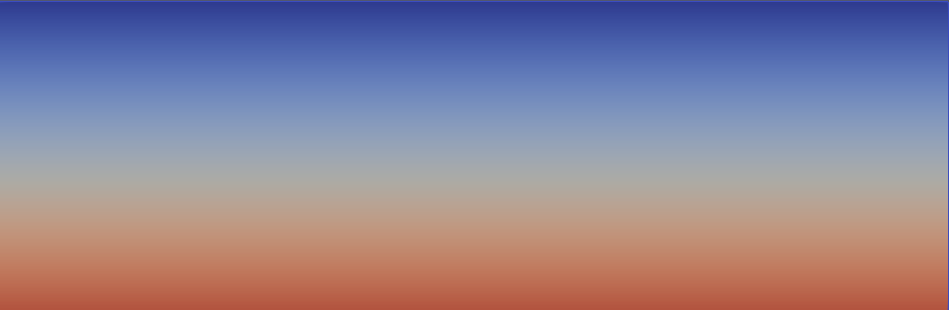
\includegraphics[scale=.3]{animation/fwi_marmousi/fwi_marmousi-00.png}}
            {animation/fwi_marmousi/out.avi}
    \end{center}
  \end{block}

  \begin{block}{Mesh evolution (constant mesh):}
    \begin{center}
      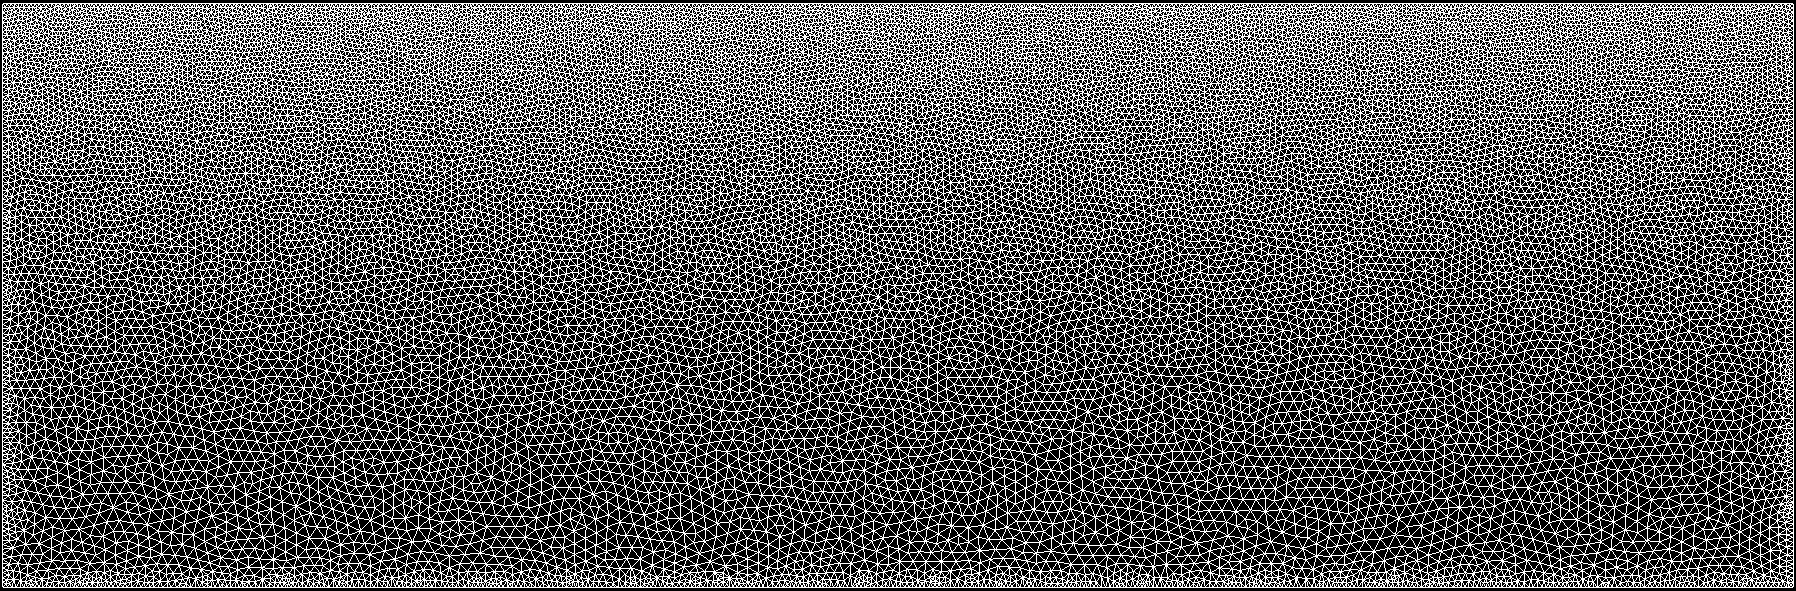
\includegraphics[scale=0.16]{animation/fwi_mesh1_black/fwi_mesh1-00.png}
    \end{center}
  \end{block}

\end{frame}


\begin{frame}[noframenumbering]{Mesh adaptation in FWI workflow}{Motivation:}
  \begin{block}{Model evolution:}
    \begin{center}
      \movie[showcontrols,loop,autostart]
            {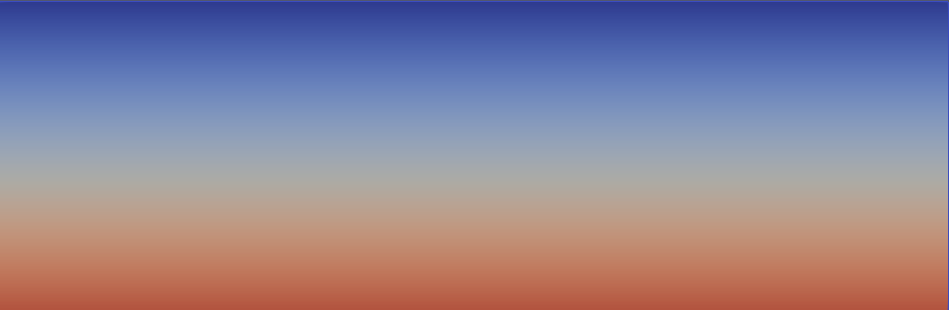
\includegraphics[scale=.3]{animation/fwi_marmousi/fwi_marmousi-00.png}}
            {animation/fwi_marmousi/out.avi}
    \end{center}
  \end{block}

  \begin{block}{Mesh evolution (model adaptative):}
    \begin{center}
            \movie[showcontrols,loop,autostart]
            {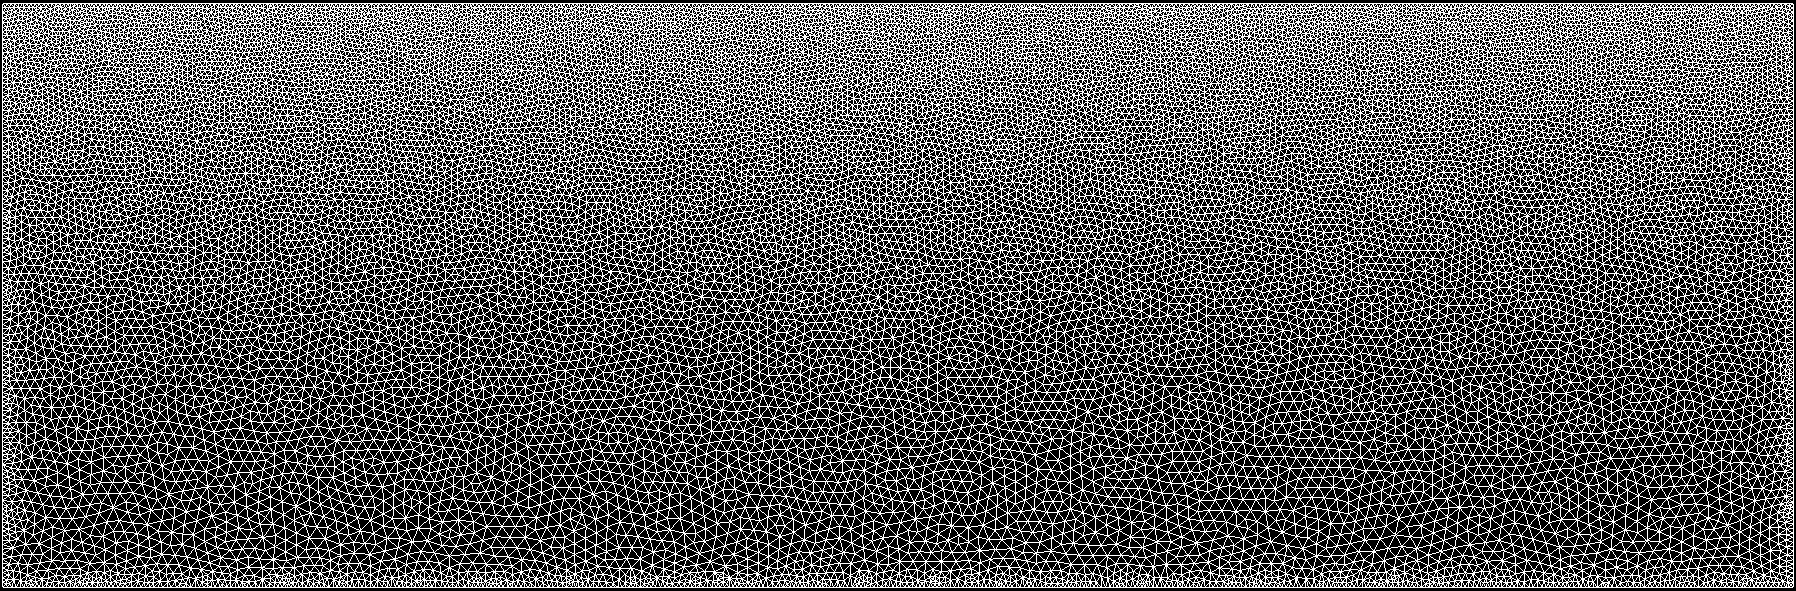
\includegraphics[scale=0.16]{animation/fwi_mesh1_black/fwi_mesh1-00.png}}
            {animation/fwi_mesh1_black/out.avi}
    \end{center}
  \end{block}
\end{frame}


\begin{frame}[noframenumbering]{Mesh adaptation in FWI workflow}{Adaptation to the velocity model}
  \begin{block}{Model evolution:}
    \begin{center}
      \movie[showcontrols,loop,autostart]
            {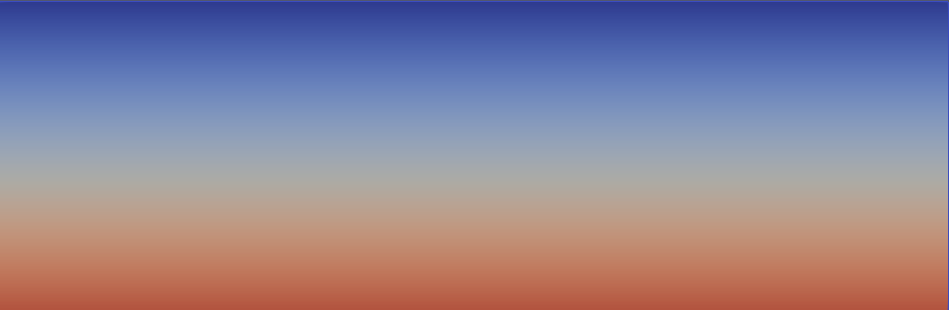
\includegraphics[scale=.3]{animation/fwi_marmousi/fwi_marmousi-00.png}}
            {animation/fwi_marmousi/out.avi}
    \end{center}
  \end{block}

  \begin{block}{Mesh evolution (model and frequency adaptative):}
    \begin{center}
            \movie[showcontrols,loop,autostart]
            {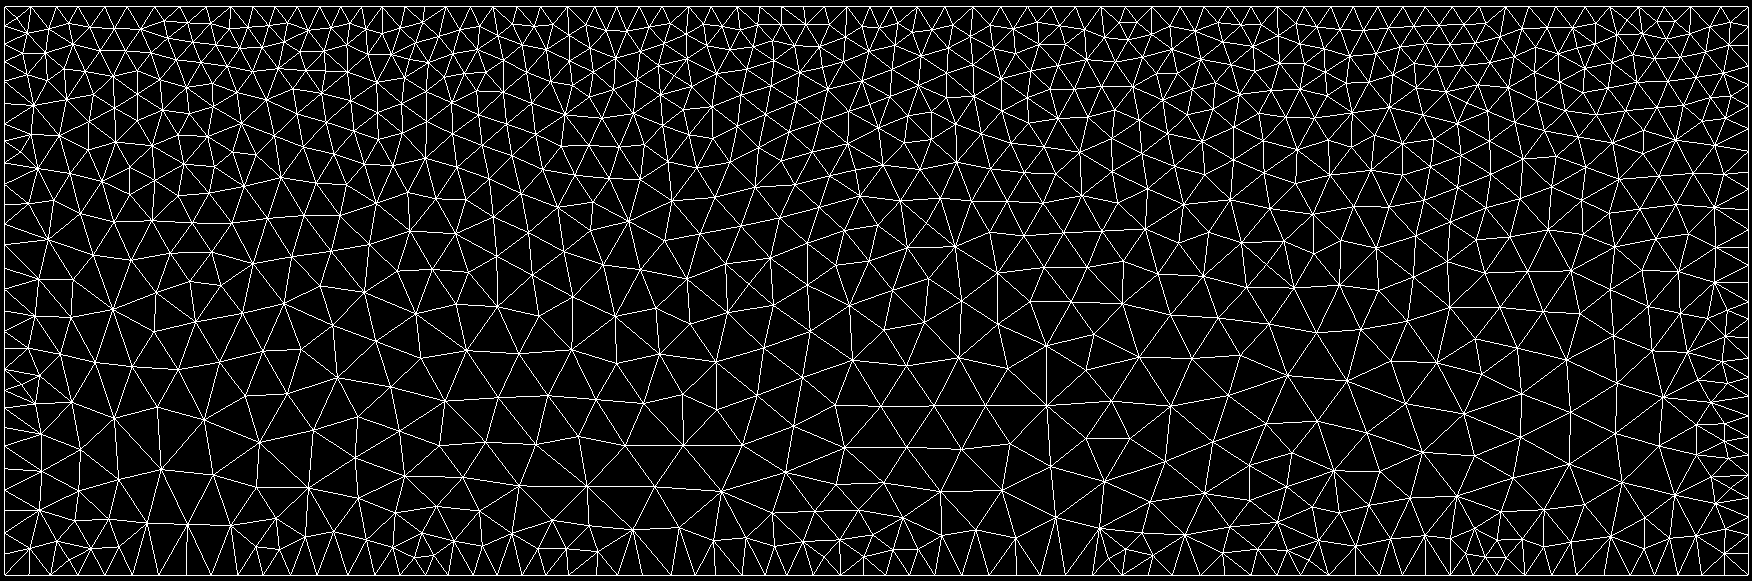
\includegraphics[scale=0.16]{animation/fwi_mesh2/fwi_mesh2-00.png}}
            {animation/fwi_mesh2/out.avi}
    \end{center}
  \end{block}
\end{frame}





% ============================================
% ====== Frame : Introduction Questions  =====
% ============================================


\begin{frame}{Mesh adaptation in FWI workflow}{Introduction}
  Why adapting the mesh in the FWI course ?
  \vspace{1cm}
  \begin{itemize}
  \item<2->{Adjust the computational burden}
  \item<3->{ Capture appearing structures}
  \item<4->{Avoid small cells in high velocity structures (\textbf{relax the CFL condition})}
  \item<5->{Enables to choose the mesh according to the frequency range currently reconstructed}
  \end{itemize}
\end{frame}



% ============================================
% ====== Frame : Proposition Ajout FWI  ======
% ============================================

\begin{frame}{Mesh adaptation in FWI workflow}{Introduction}
  How to include mesh adaptation into FWI workflow ?
\begin{figure}[!htbp]
\centering
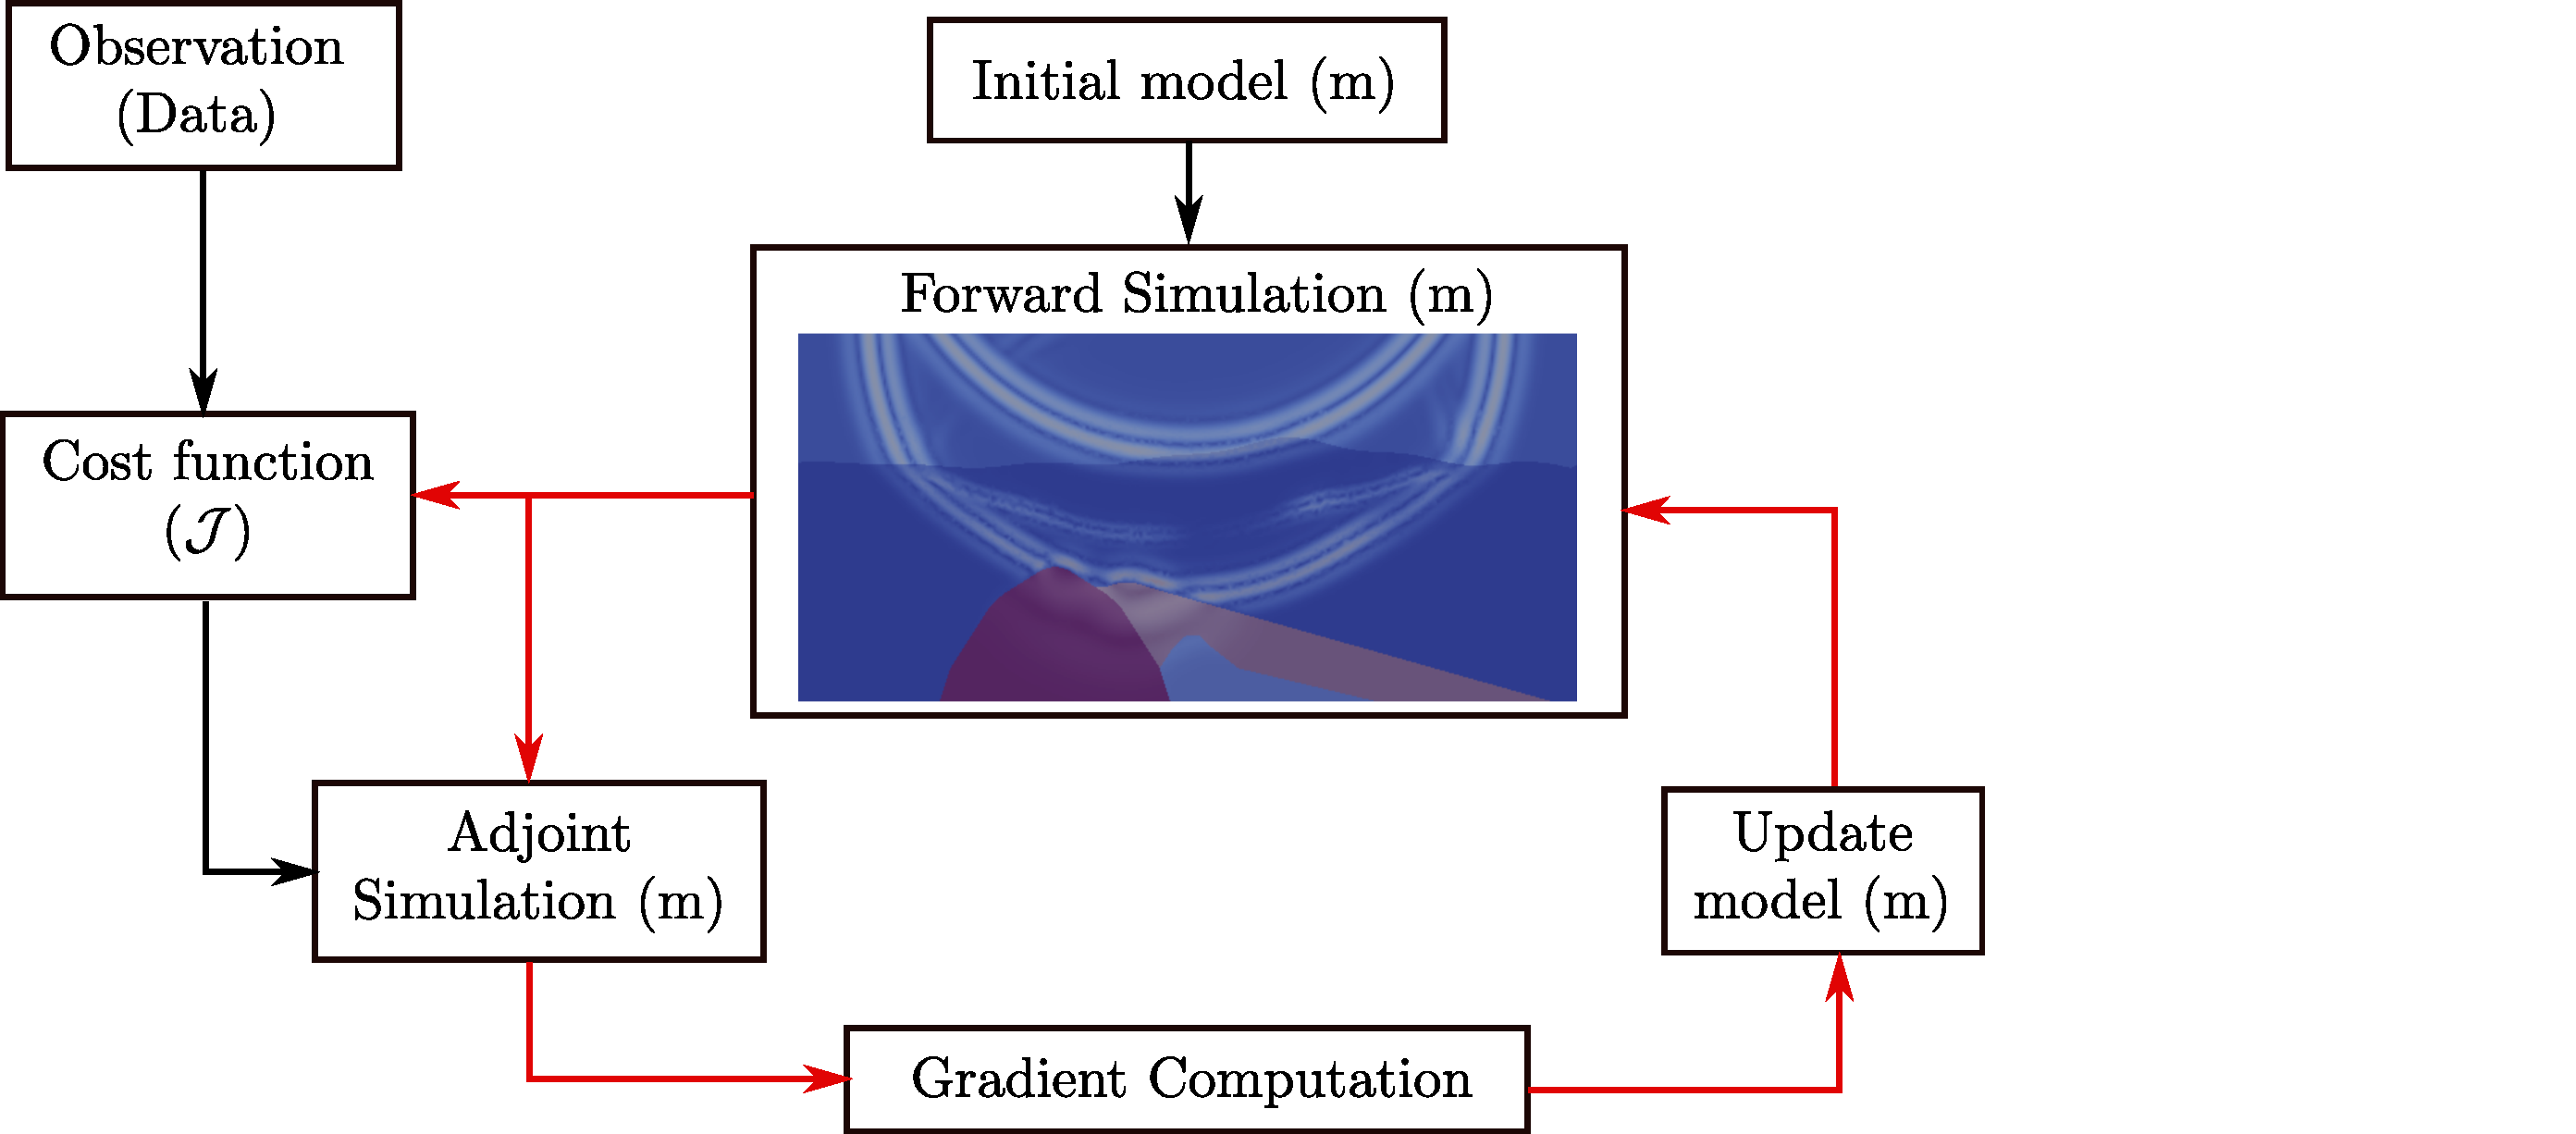
\includegraphics[scale=0.2]{image/fwi_workflow_mesh_adapt0.pdf}
\caption{FWI workflow extended with mesh adaptation.}
\label{fwi_workflow_mesh_extended}
\end{figure}
\end{frame}


\begin{frame}[noframenumbering]{Mesh adaptation in FWI workflow}{Introduction}
  How to include mesh adaptation into FWI workflow ?
\begin{figure}[!htbp]
\centering
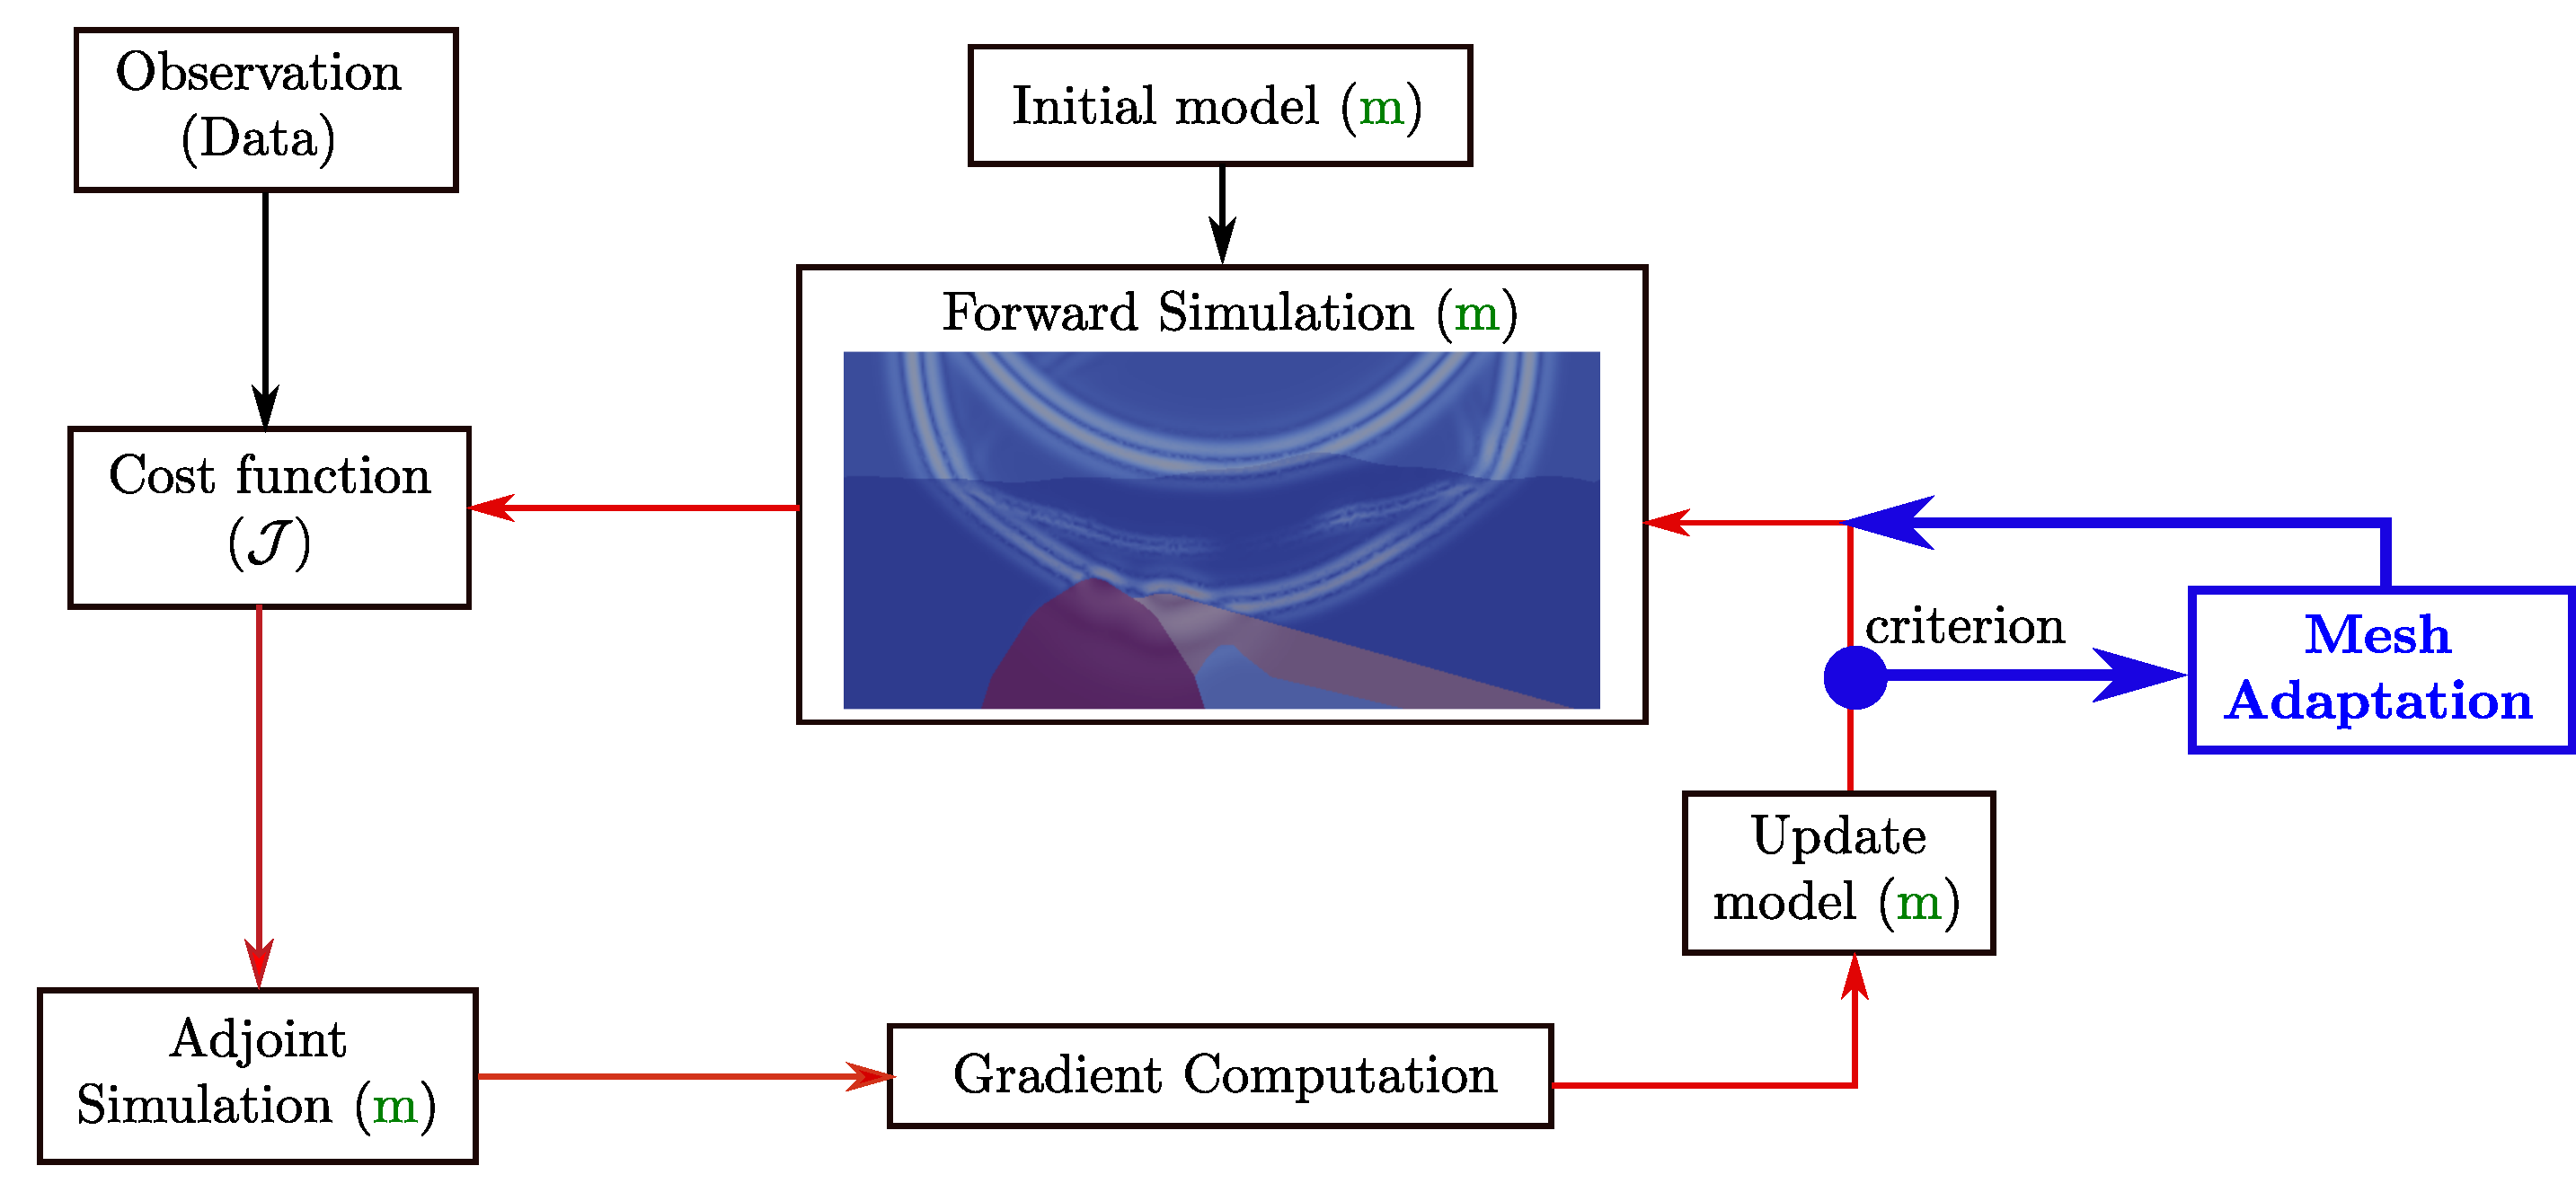
\includegraphics[scale=0.2]{image/fwi_workflow_mesh_adapt.pdf}
\caption{FWI workflow extended with mesh adaptation.}
\label{fwi_workflow_mesh_extended}
\end{figure}
\end{frame}



% =========================================================
% ====== Frame : Mesh adaptation classical workflow  ======
% =========================================================

\setbeamercovered{invisible}
\subsection{Mesh Adaptation principle}

\begin{frame}{Mesh Adaptation}{Definitions}
  $\boldsymbol{S^i}$ : solution at the $i^{th}$ iteration |
  $\boldsymbol{\Triangles^i}$ : mesh at the $i^{th}$ iteration
  \vspace{0.5cm}
   \begin{figure}
     \begin{tikzpicture}
       \node[anchor=south west,inner sep=0] at (0,0) {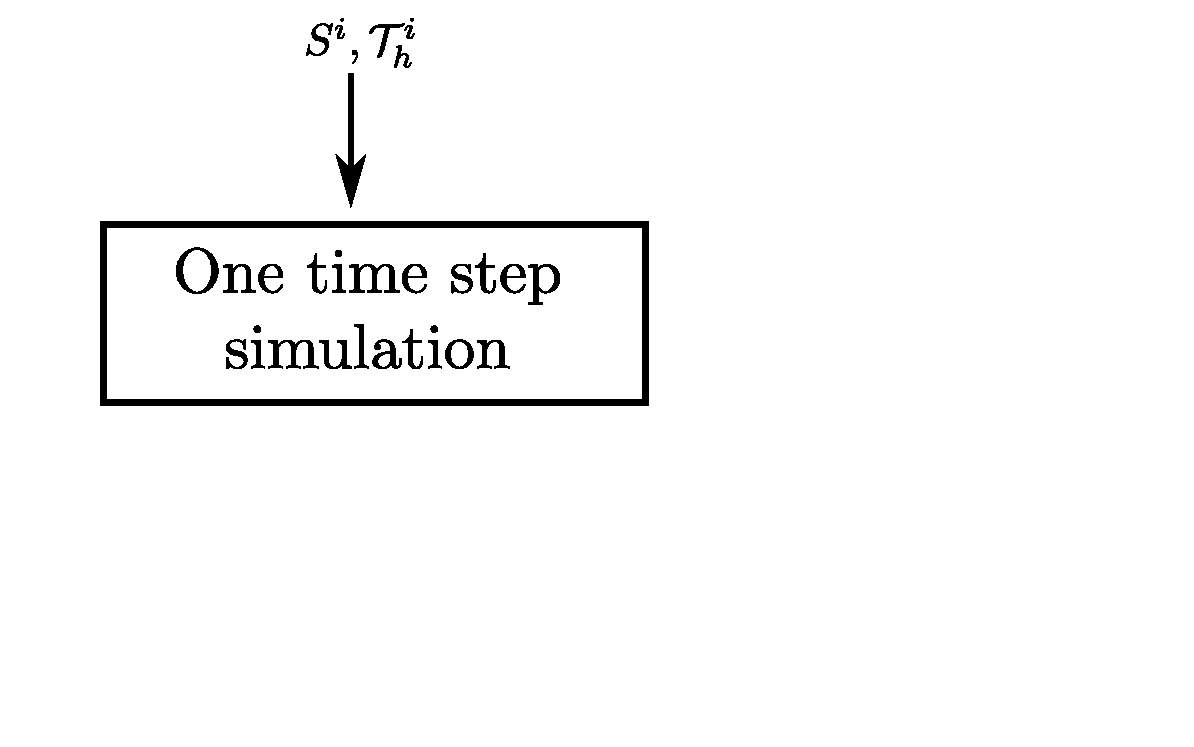
\includegraphics[width=0.8\textheight]{image/mesh_adapt_workflow5.pdf}};
        \end{tikzpicture}
        \caption{Classical mesh adaptation workflow.}
   \end{figure}
\end{frame}


\begin{frame}[noframenumbering]{Mesh Adaptation}{Definitions}
  $\boldsymbol{S^i}$ : solution at the $i^{th}$ iteration |
  $\boldsymbol{\Triangles^i}$ : mesh at the $i^{th}$ iteration
  \vspace{0.5cm}
   \begin{figure}
     \begin{tikzpicture}
       \node[anchor=south west,inner sep=0] at (0,0) {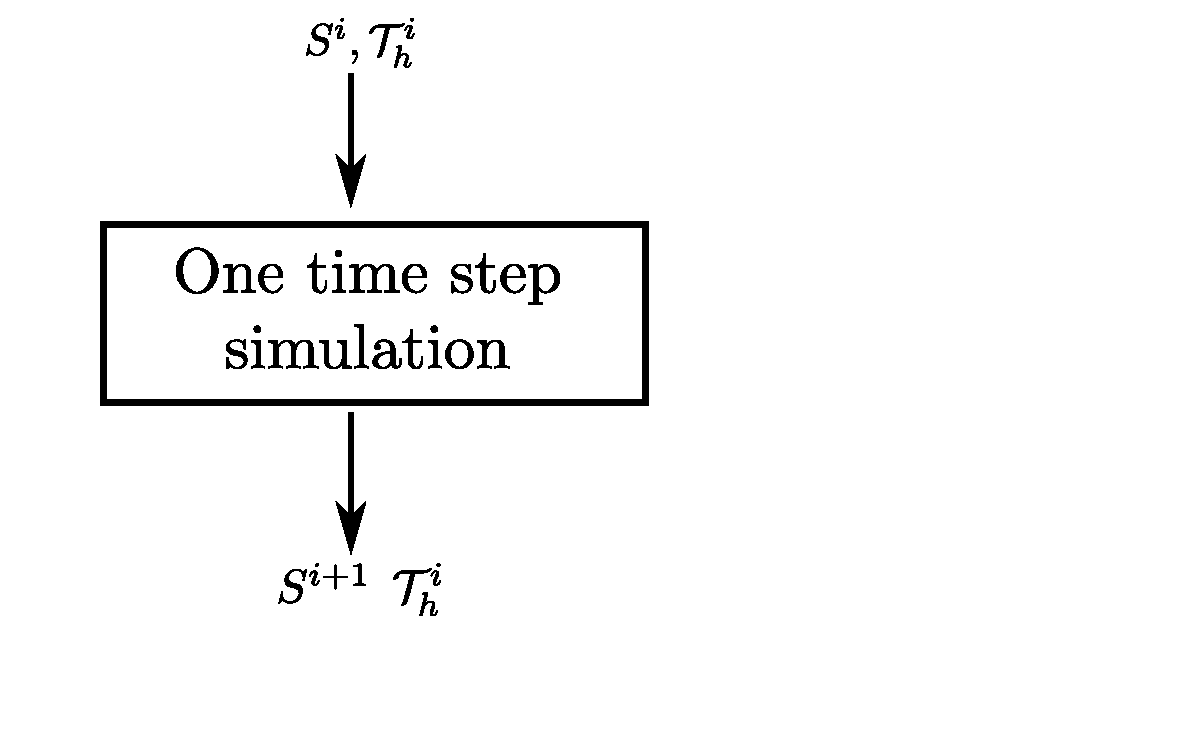
\includegraphics[width=0.8\textheight]{image/mesh_adapt_workflow4.pdf}};
        \end{tikzpicture}
        \caption{Classical mesh adaptation workflow.}
   \end{figure}
\end{frame}


\begin{frame}[noframenumbering]{Mesh Adaptation}{Definitions}
  $\boldsymbol{S^i}$ : solution at the $i^{th}$ iteration |
  $\boldsymbol{\Triangles^i}$ : mesh at the $i^{th}$ iteration
  \vspace{0.5cm}
   \begin{figure}
     \begin{tikzpicture}
       \node[anchor=south west,inner sep=0] at (0,0) {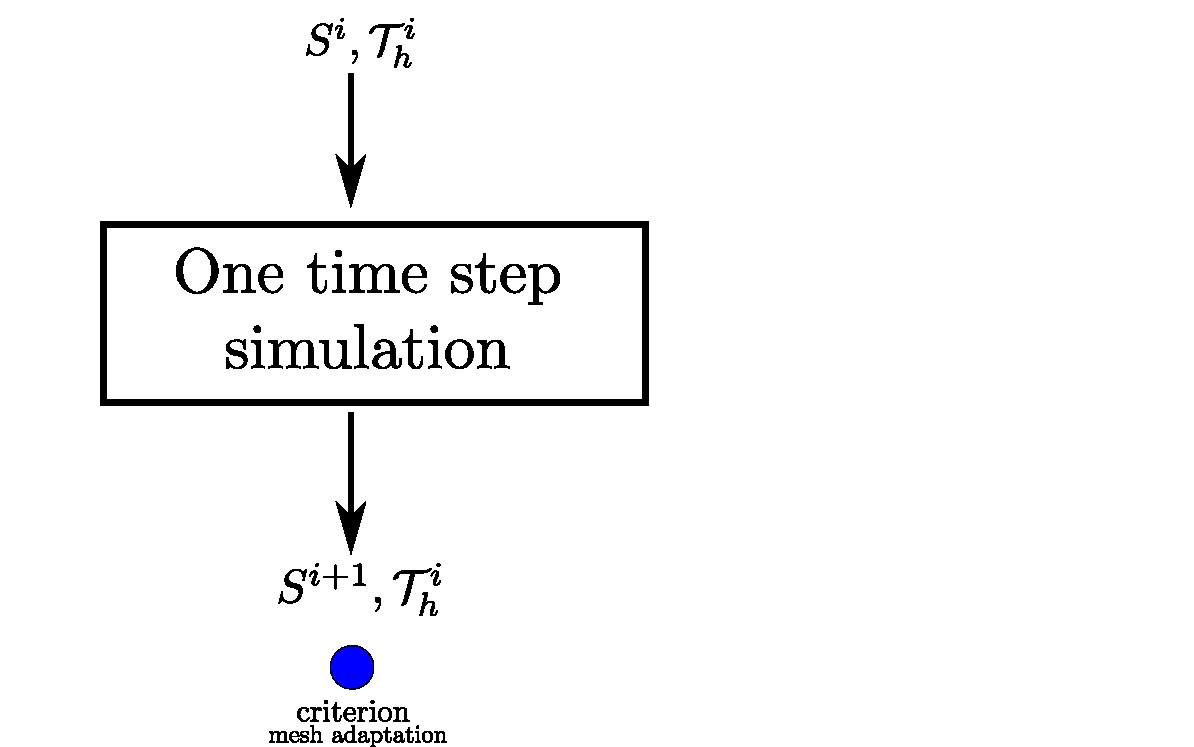
\includegraphics[width=0.8\textheight]{image/mesh_adapt_workflow3.pdf}};
        \end{tikzpicture}
        \caption{Classical mesh adaptation workflow.}
   \end{figure}
\end{frame}


\begin{frame}[noframenumbering]{Mesh Adaptation}{Definitions}
  $\boldsymbol{S^i}$ : solution at the $i^{th}$ iteration |
  $\boldsymbol{\Triangles^i}$ : mesh at the $i^{th}$ iteration
  \vspace{0.5cm}
   \begin{figure}
     \begin{tikzpicture}
       \node[anchor=south west,inner sep=0] at (0,0) {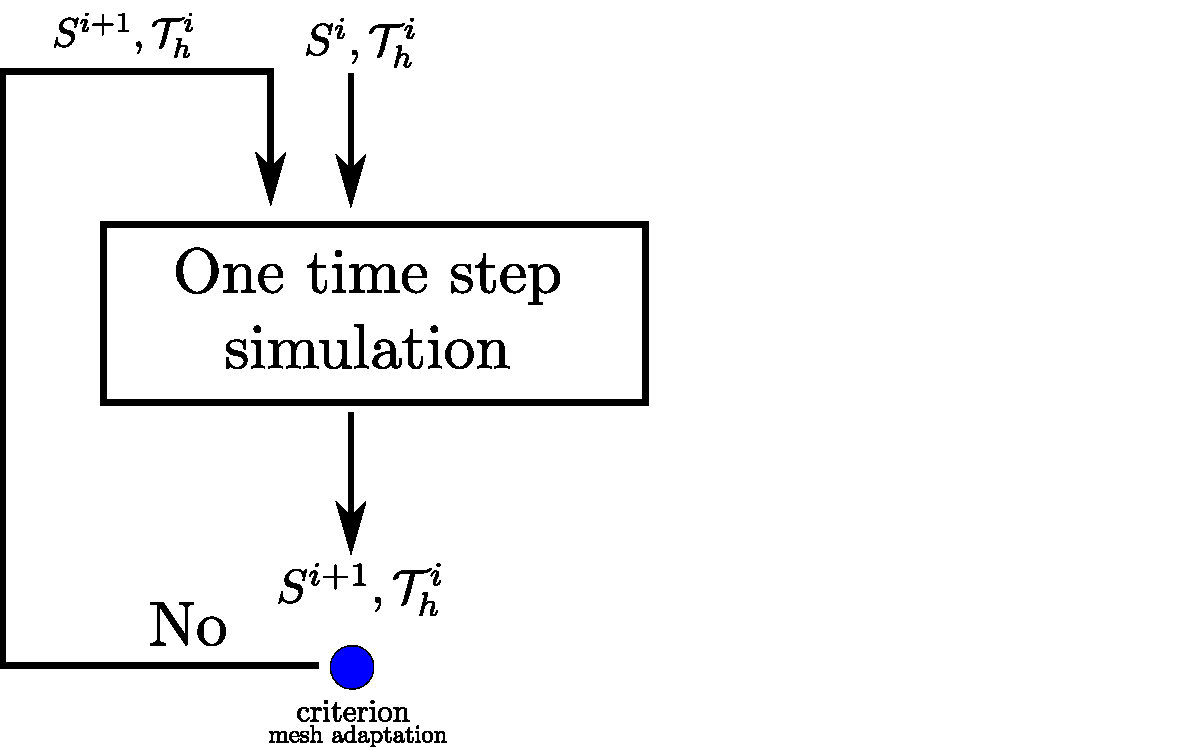
\includegraphics[width=0.8\textheight]{image/mesh_adapt_workflow2.pdf}};
        \end{tikzpicture}
        \caption{Classical mesh adaptation workflow.}
   \end{figure}
\end{frame}


\begin{frame}[noframenumbering]{Mesh Adaptation}{Definitions}
  $\boldsymbol{S^i}$ : solution at the $i^{th}$ iteration |
  $\boldsymbol{\Triangles^i}$ : mesh at the $i^{th}$ iteration
  \vspace{0.5cm}
   \begin{figure}
     \begin{tikzpicture}
       \node[anchor=south west,inner sep=0] at (0,0) {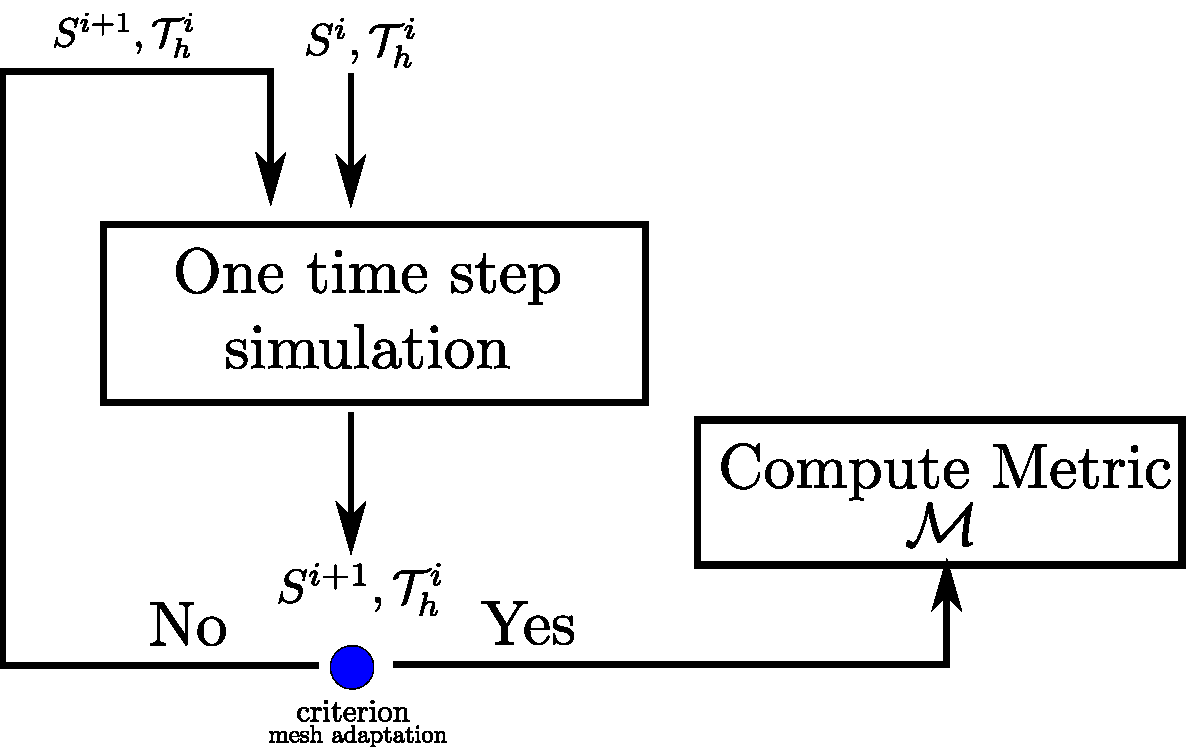
\includegraphics[width=0.8\textheight]{image/mesh_adapt_workflow1.pdf}};
        \end{tikzpicture}
        \caption{Classical mesh adaptation workflow.}
   \end{figure}
\end{frame}


\begin{frame}[noframenumbering]{Mesh Adaptation}{Definitions}
  $\boldsymbol{S^i}$ : solution at the $i^{th}$ iteration |
  $\boldsymbol{\Triangles^i}$ : mesh at the $i^{th}$ iteration
  \vspace{0.5cm}
   \begin{figure}
     \begin{tikzpicture}
       \node[anchor=south west,inner sep=0] at (0,0) {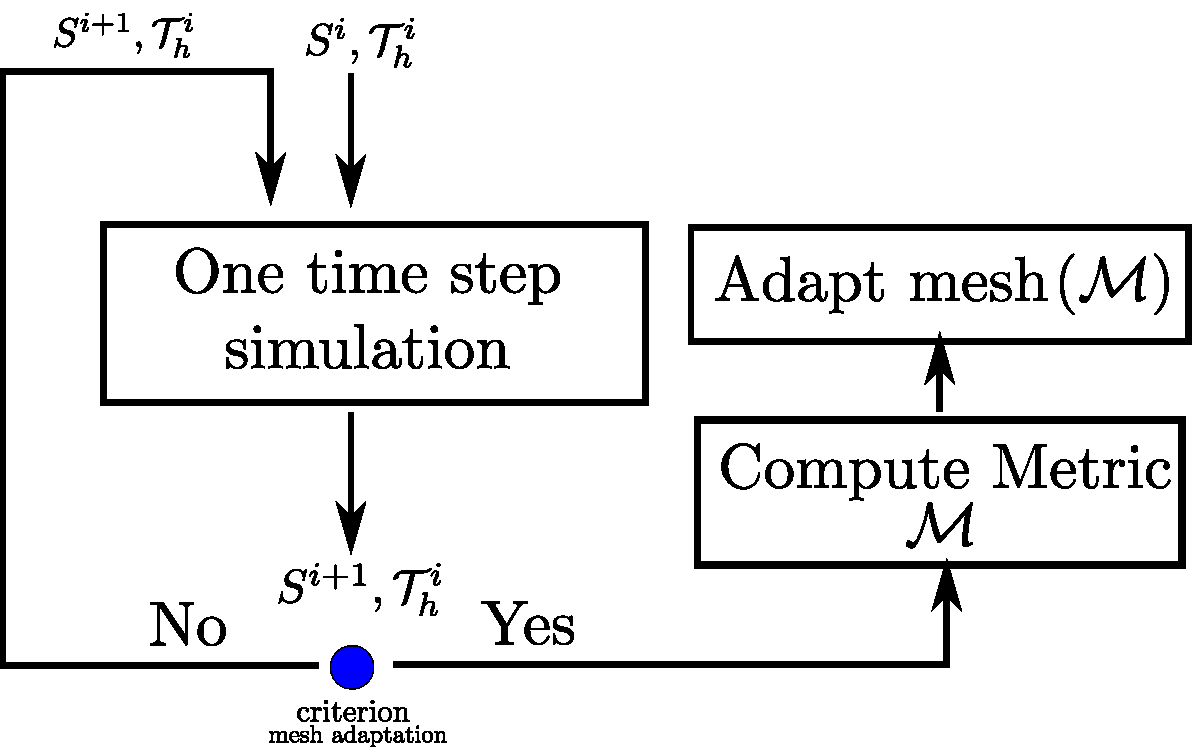
\includegraphics[width=0.8\textheight]{image/mesh_adapt_workflow6.pdf}};
        \end{tikzpicture}
        \caption{Classical mesh adaptation workflow.}
   \end{figure}
\end{frame}


\begin{frame}[noframenumbering]{Mesh Adaptation}{Definitions}

  $\boldsymbol{S^i}$ : solution at the $i^{th}$ iteration |
  $\boldsymbol{\Triangles^i}$ : mesh at the $i^{th}$ iteration

  \vspace{0.5cm}
   \begin{figure}
     \begin{tikzpicture}
       \node[anchor=south west,inner sep=0] at (0,0) {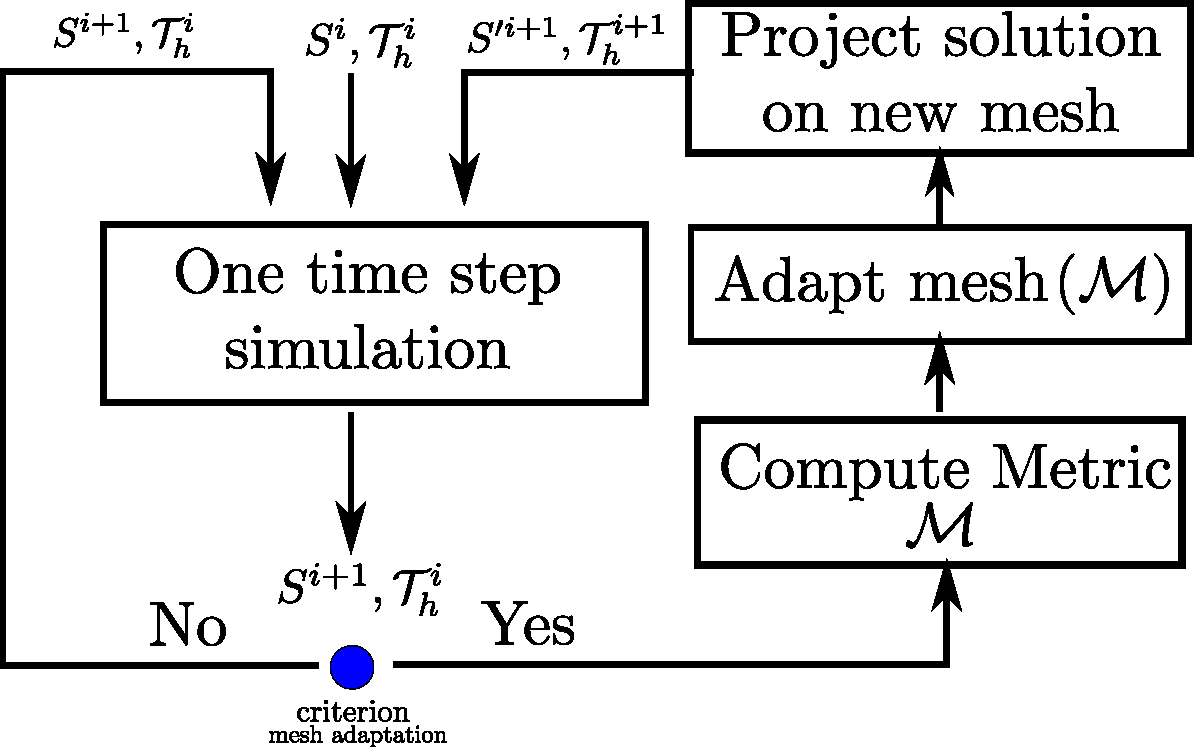
\includegraphics[width=0.8\textheight]{image/mesh_adapt_workflow.pdf}};
        \uncover<2->{
        \node at (8.0,1.52) {\textbf{\textcolor{blue}{Mshmet \footcite{Mshmet}}}};
        \node at (7.8,2.64) {\textbf{\textcolor{red}{MMG \footcite{Mmg}}}};
          \draw [blue,ultra thick,rounded corners] (3.9,0.95) rectangle (6.95,2.0);
          \draw [red,ultra thick,rounded corners] (3.9,2.25) rectangle (6.95,3.1);}
        \end{tikzpicture}
        \caption{Classical mesh adaptation workflow.}
   \end{figure}
\end{frame}








% ============================================
% ====== Frame : Some definitiions      ======
% ============================================

\begin{frame}{Some Definitions}
  \vspace{-0.1cm}
  \uncover<2->{
  \begin{block}{Metric definition:}
    \small
    $\forall P \in \Domain, \boldsymbol{\metric(P)}$ is a \textbf{SPD matrix} of size $\dim \times \dim$.

      \begin{empheq}{align}
    \forall (P,M) \in \Domain^2, \parallel\vec{PM} \parallel^2_{\metric(P)} &= \langle \vec{PM}, \metric(P) \vec{PM} \rangle \\
                              %\parallel\vec{PM} \parallel_{\metric(P)}   &= \sqrt{\vec{PM}^\top \metric(P) \vec{PM}}
      \end{empheq}
      \end{block}
}
  \uncover<3->{
    \vspace{-0.1cm}
  \begin{block}{Unit ball : Set of point $M$ such that $\parallel \vec{PM} \parallel_{\metric(P)} = 1.$}
    \small
          \begin{empheq}{align}
   \text{In 2D :  } \metric(P) = S \Lambda S^\top\,, \Lambda =  \begin{pmatrix}
    \lambda_{1} &\\
    & \lambda_2
  \end{pmatrix}\,, \lambda_1 \geq \lambda_2 > 0.
          \end{empheq}
          \begin{multicols}{2}
            \begin{figure}[!htbp]
\centering
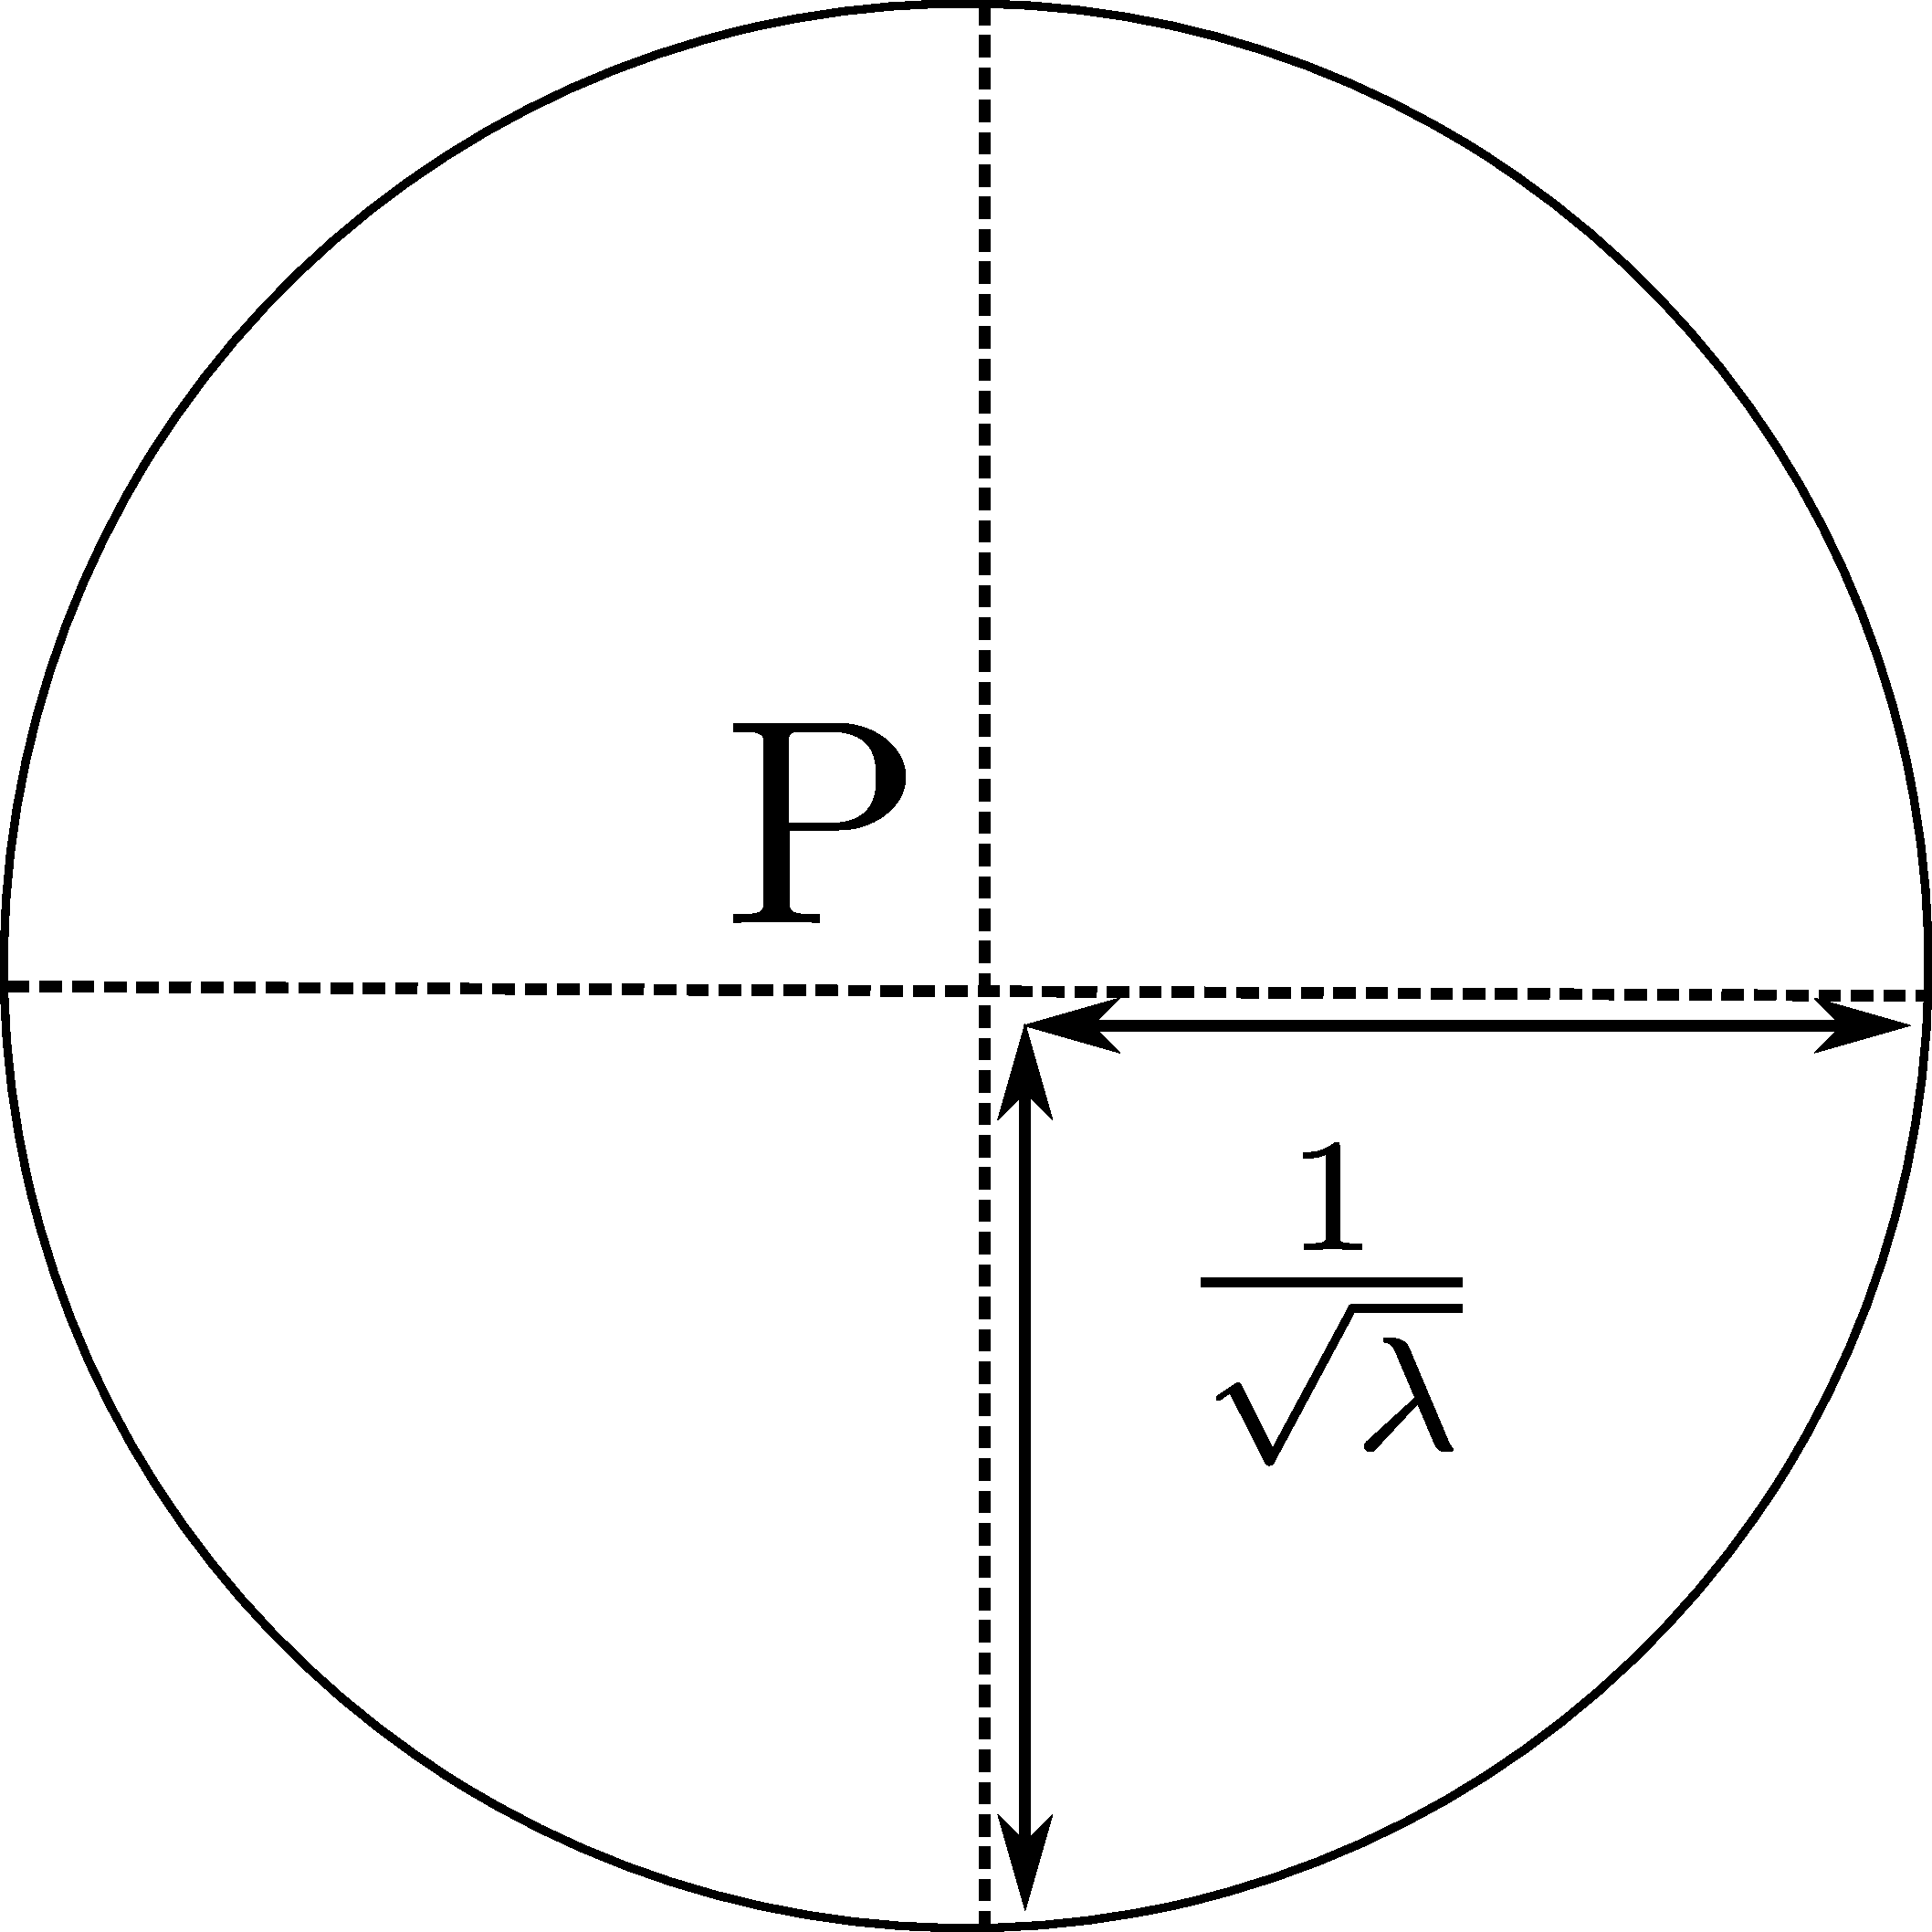
\includegraphics[scale=0.04]{image/ellipse_iso_triangle.pdf}
\vspace{0.2cm}
\caption{\tiny{Unit ball $(\lambda_1 = \lambda_2 = \lambda)$}}
\label{ellipse_iso_triangle}
\end{figure}
            \columnbreak
           \begin{figure}[!htbp]
\centering
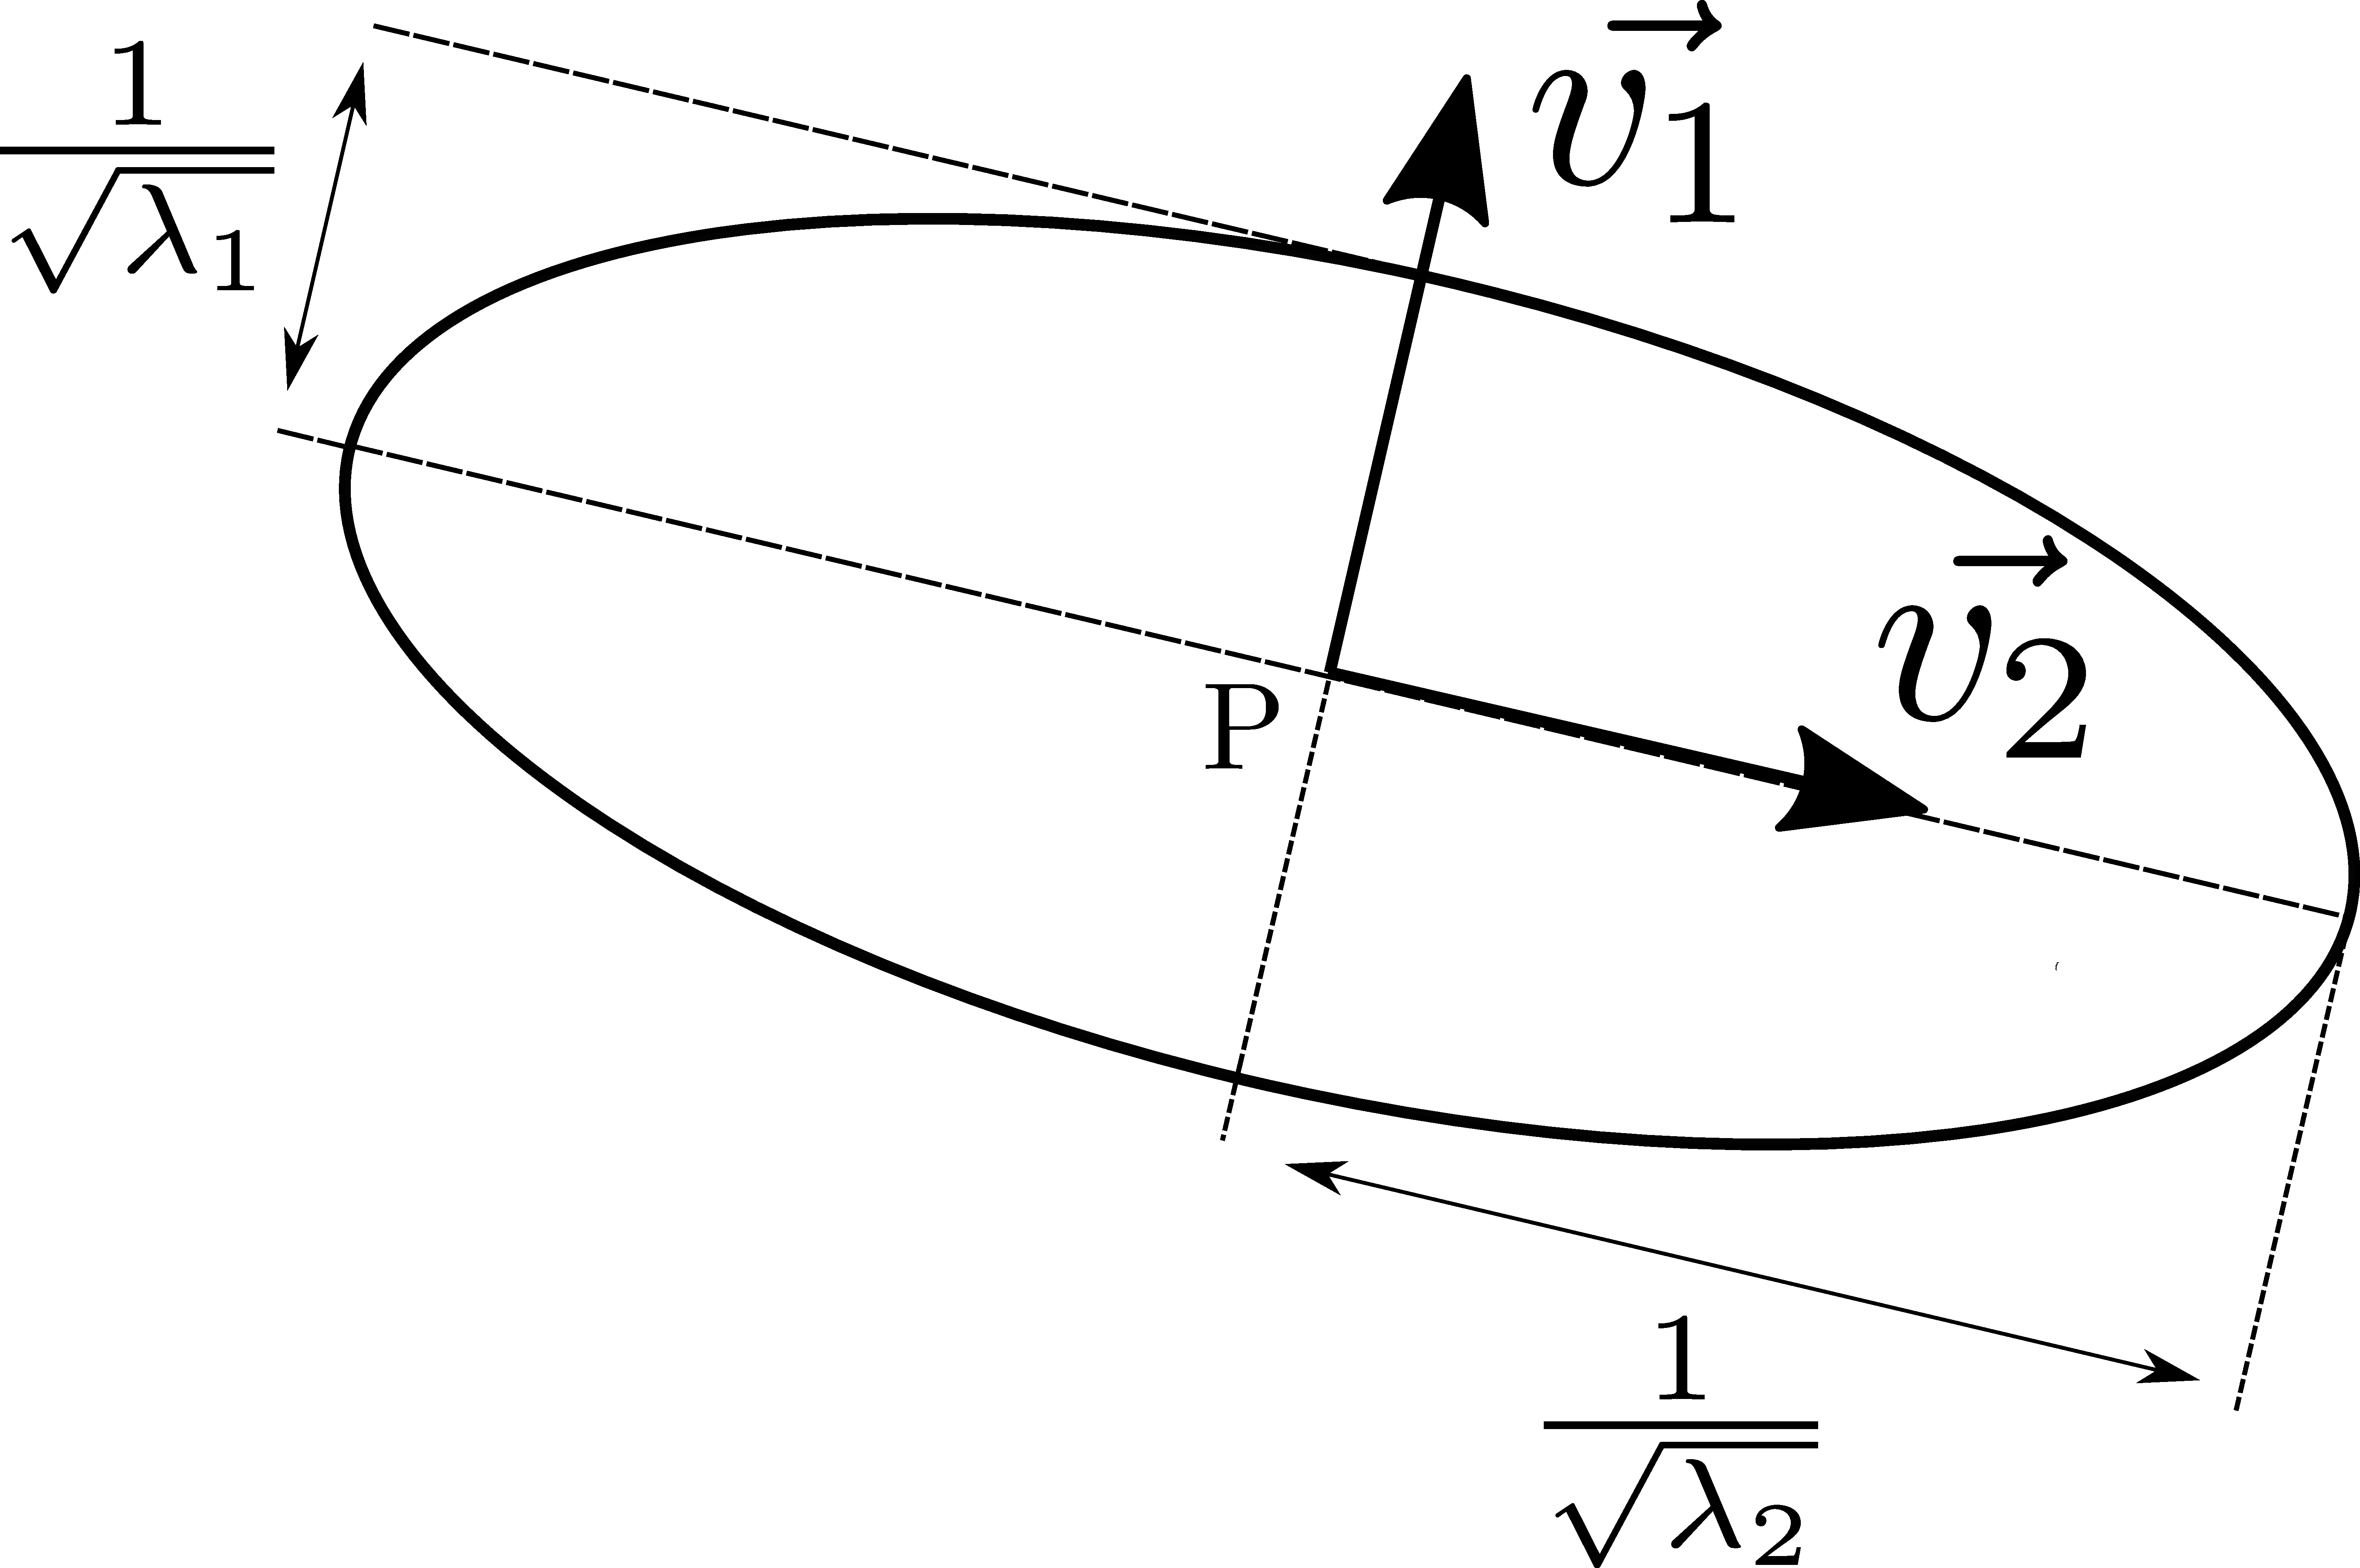
\includegraphics[scale=0.028]{image/ellipse_aniso.pdf}
\vspace{-0.3cm}
\caption{\tiny{Unit ball $(\lambda_1 >> \lambda_2)$}}
\label{ellipse_iso_triangle}
     \end{figure}
 \end{multicols}
  \end{block}
  }
\end{frame}




% ============================================
% ====== Frame : Control the error      ======
% ============================================

\begin{frame}{Control the interpolation error}
  \small
  [P.J. Frey and F. Alauzet]\footcite{freyAnisotropicMeshAdaptation2005}: control the error on the element $\element$:
\vspace{-0.1cm}
  \begin{multicols}{2}
  \begin{empheq}{align}
\exists \, \bar{\metric}(\element)\, / \, \varepsilon_\element = \underset{\overrightarrow{e}\in E_\element}{max} \langle \overrightarrow{e}, \bar{\metric}(\element) \overrightarrow{e} \rangle. \label{error_frey}
  \end{empheq}
  \columnbreak
  \begin{figure}
    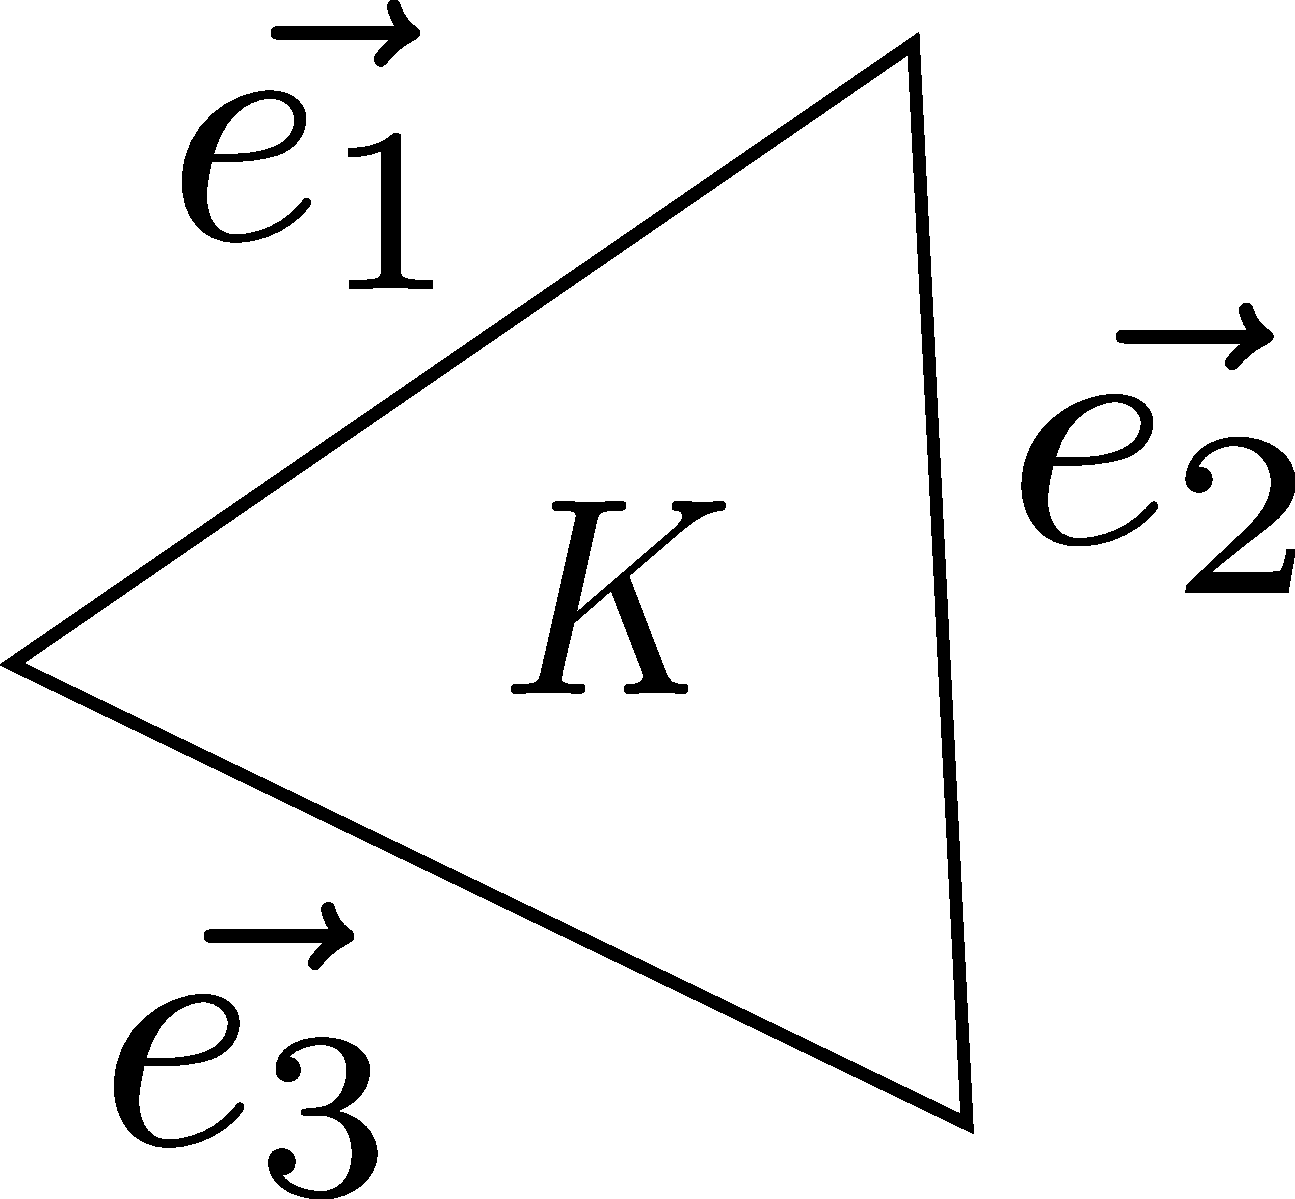
\includegraphics[scale=0.07]{image/triangle_error_frey}
%    \caption{Element $K$}
    \end{figure}
  \end{multicols}

  \uncover<2->{
  \vspace{-0.8cm}
  \begin{block}{Objective:}
    Adapt $\Triangles$ into $\Triangles$' such that:

    \begin{empheq}{align}
      \varepsilon &= \langle \overrightarrow{e}, \bar{\metric}(\element) \overrightarrow{e} \rangle \,, \qquad \forall \element \in \Triangles'\,, \qquad \forall \overrightarrow{e} \in E_\element. \\
            & \qquad \qquad \qquad \text{with:  } \metric = \frac{1}{\varepsilon} \bar{\metric}. \\
      1 &= \langle \overrightarrow{e}, \metric(\element) \overrightarrow{e} \rangle \,, \qquad \forall \element \in \Triangles'\,, \qquad \forall \overrightarrow{e} \in E_\element.
    \end{empheq}
  \end{block}
}

  \end{frame}



% ============================================
% ====== Frame : Algorithm principle    ======
% ============================================

%\setbeamercovered{transparent}
\begin{frame}{Mesh adaptation Algorithm}

  \begin{block}{Distance between $P$ and $M$ according to the metric field $\metric$:}
  \begin{empheq}{align}
\parallel \overrightarrow{PM} \parallel_\metric =  \int_{0}^{1} \sqrt{ \overrightarrow{PM}^\top  \metric( (1-t)P + tM) \overrightarrow{PM}  } \, dt \,.
  \end{empheq}
  \end{block}

  \begin{enumerate}
    \uncover<2->{
\item Scan all the edges $\overrightarrow{PM}$ and verify $\parallel \overrightarrow{PM} \parallel_\metric=1$:
\begin{itemize}
\item{Split the current edge if too long;}
\item{Collapse the edge if too short.}
\end{itemize}
    }
    \uncover<3->{
\item Check quality of the elements:
\begin{itemize}
\item Swap edges if "too bad elements";
\item{Move points.}
\end{itemize}
    }
    \uncover<3-4>{
\begin{tikzpicture}[remember picture,overlay]
    \node[xshift=80mm,yshift=-56mm,anchor=north west] at (current page.north west){%
    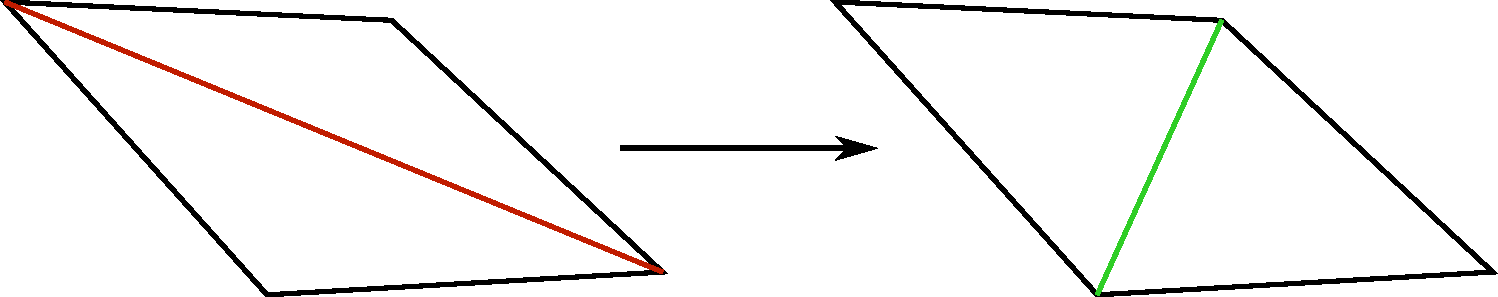
\includegraphics[width=40mm]{image/swap_edge.pdf}};
\end{tikzpicture}
}
    \uncover<4->{
      \vspace{-0.5cm}
    \item Go to 1. until convergence of the algorithm:
      \begin{empheq}{align}
        \frac{\sqrt{2}}{2} \le \parallel \overrightarrow{PM} \parallel_\metric \le \sqrt{2}\,.
      \end{empheq}
      }
\end{enumerate}

\end{frame}

%% %% \begin{frame}
%% %%   \begin{block}{Definition of Isotropic/ Anisotropic cells}
%% %% \begin{multicols}{2}
%% %%   \begin{figure}[H]
%% %% 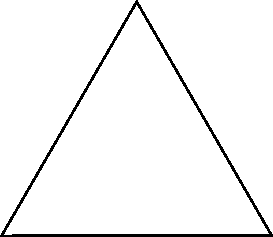
\includegraphics[scale=0.6]{image/isotropic_cell.pdf}
%% %% \caption{Isotropic cell  ($\lambda_1 = \lambda_2$).}
%% %% \end{figure}
%% %% \columnbreak
%% %% \begin{figure}
%% %% 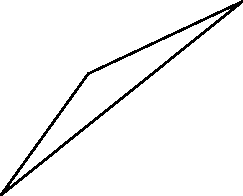
\includegraphics[scale=0.7]{image/anisotropic_cell.pdf}
%% %% \caption{Anisotropic cell ($\lambda_1 >> \lambda_2$).}
%% %% \end{figure}
%% %% \end{multicols}
%% %% \end{block}
%% %% \end{frame}




% ============================================
% ====== Frame : How to define the metric  ===
% ============================================
\subsection{Adaptation according to the physical parameters}
\begin{frame}{Define a metric according to the physical parameters}
  How to define a metric according to $\smodel^i$ instead of $S^i$ ?
  \vspace{0.5cm}
  \begin{multicols}{2}
    \vspace{-1cm}
    \begin{figure}
      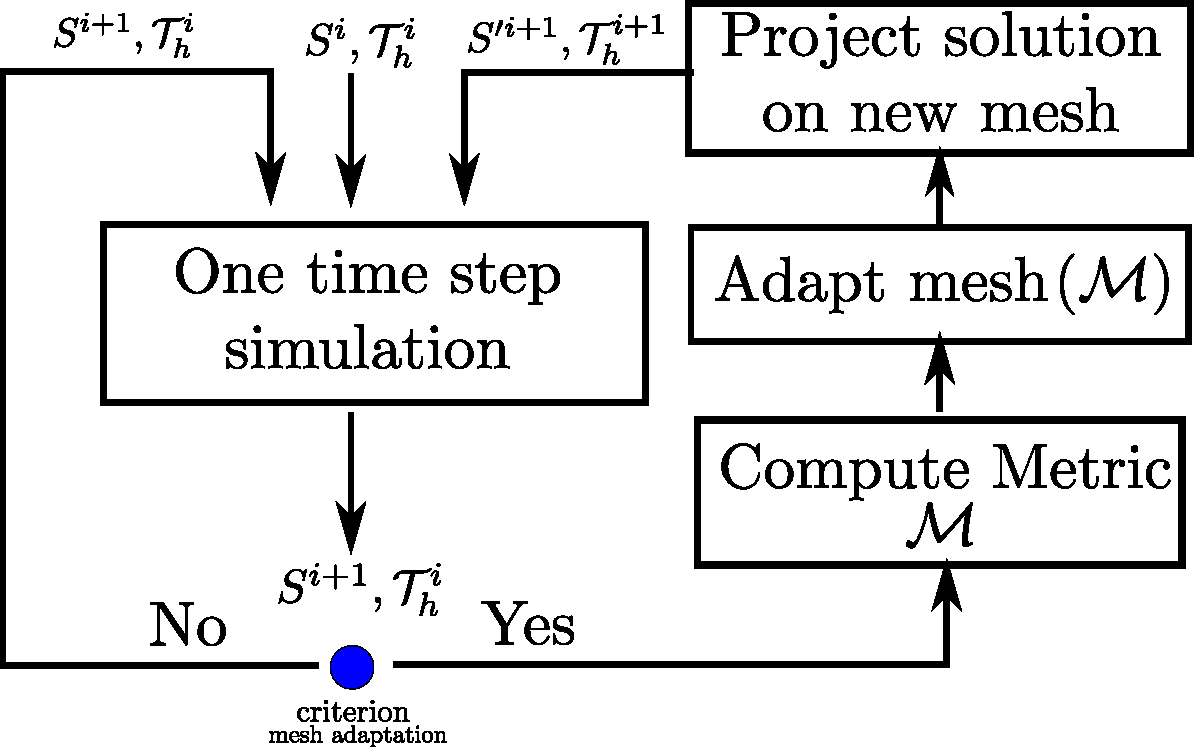
\includegraphics[scale=0.27]{image/mesh_adapt_workflow.pdf}
    \end{figure}
    \columnbreak
        \begin{figure}
      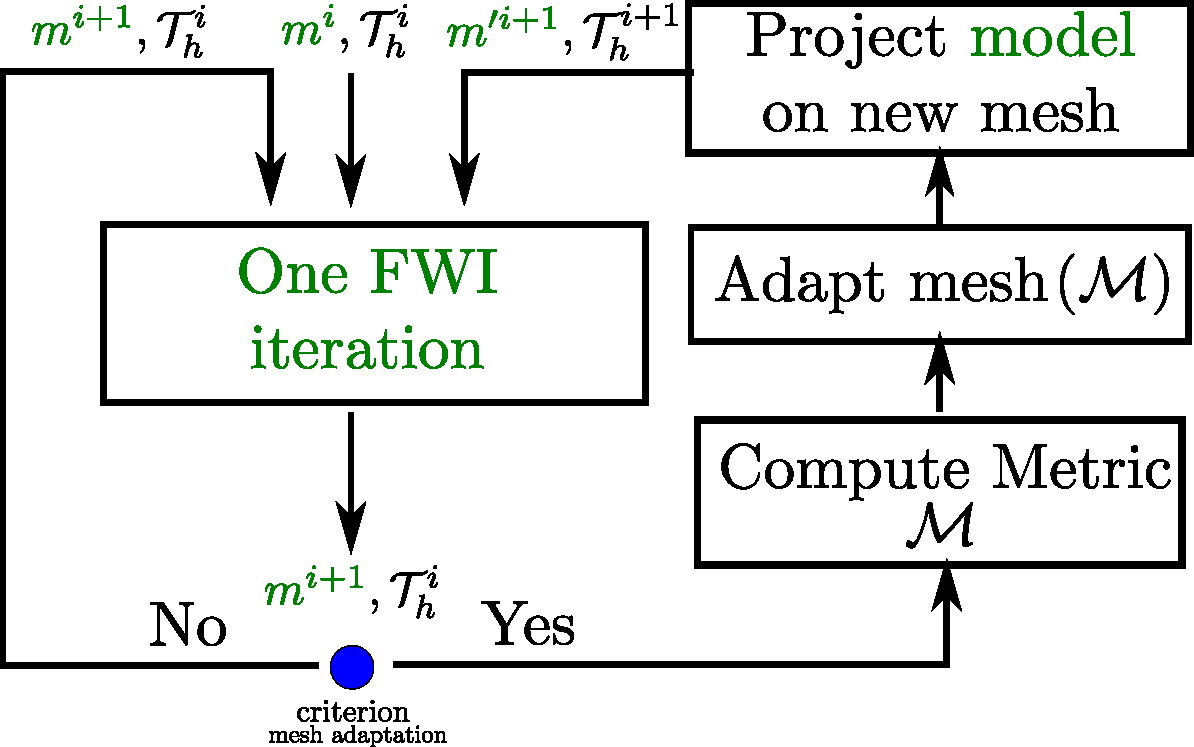
\includegraphics[scale=0.27]{image/mesh_adapt_workflow_fwi.pdf}
    \end{figure}
     \end{multicols}
\end{frame}


\begin{frame}[noframenumbering]{Define a metric according to the model parameters}
  \small
  No predominant directions $\longrightarrow$ Isotropic metric ($\metric(x) \approx h(x)$)

  \uncover<2->{
  In a reference square of size $\lambda \times \lambda$:
  \begin{empheq}{align}
    \nppw^2  &= \frac{\lambda^2}{a} \frac{(\PolOrder + 1)(\PolOrder + 2)}{2}, \text{  where: } \lambda = \velocity / \fmax
  \end{empheq}
  }

  \uncover<3->{
  Isotropic cell hypothesis:
  \begin{empheq}{align}
    a = \frac{\sqrt{3}}{4} h^2
  \end{empheq}
  }

  \uncover<4->{
  \begin{block}{Heuristic size map formula:}
  \begin{empheq}{align}
  \forall x \in \Domain, \, \,  h(x)=2\frac{\lambda(x)}{\nppw}\sqrt{\frac{(\PolOrder+1)(\PolOrder+2)}{2\sqrt{3}}} \,.
  \end{empheq}
  \end{block}
  }
\end{frame}




% ============================================
% ====== Frame : Find NPPW  ==================
% ============================================

\begin{frame}{Numerical assessement of the isotropic size map}{Determine the $\nppw$ value}
  \begin{multicols}{2}
    \begin{itemize}
    \item 2s simulation
    \item 1 source: First order ricker $\fpeak=10$Hz
    \item 462 receivers
    \item Constant velocity model (to avoid errors from mis-representation of the model)
    \item compare numerical traces with analytic traces \footcite{gar6more}
    \item for various $\nppw$ values
    \end{itemize}
    \columnbreak
  \begin{figure}[H]
  \centering
  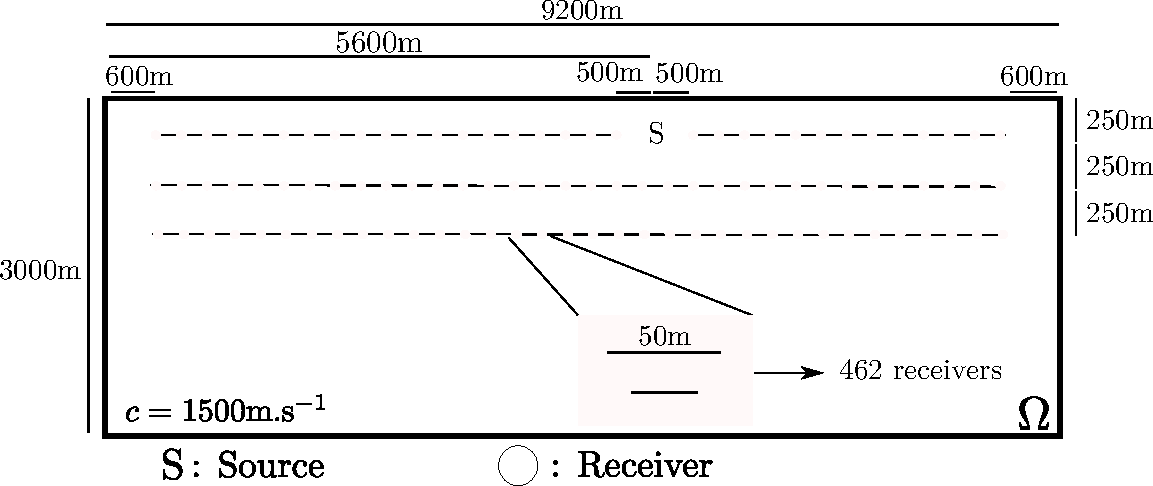
\includegraphics[scale=0.31]{image/precision_test.pdf}
  \caption{Experimental setup for the accuracy assessment.}
  \label{homogeneous_prec}
  \end{figure}
  \end{multicols}
  \end{frame}


% ============================================
% ====== Frame : Graph error / nppw  =========
% ============================================

\begin{frame}{Error as a function of $\nppw$}
  \begin{figure}[H]
 \vspace{-0.3cm}
\centering
 \setlength{\plotwidth}{10cm}
    \setlength{\plotheight}{6.0cm}
    \begin{tikzpicture}
      \begin{axis}[%
          width=\plotwidth, height=\plotheight,,
          at={(0,0)},scale only axis,separate axis lines,
          ymode=log,
          xlabel={$\nppw$},
          ylabel={error},
          grid=both,
          grid style={line width=.1pt, draw=gray!10},
          major grid style={line width=.2pt,draw=gray!50},
          %%   ymode=log,
          %yminorticks=true,
          %% xmin=0,xmax=35,
          %% ymin=0,ymax=1.25,
          legend pos=north east
          %ymin=0.98,ymax=1.22
        ]

        %% load current data
        %% -----------------
        \addplot[color=blue!50!black,mark options={solid}, mark=triangle*,
          line width=1pt,
          mark size=2pt]
        table[x=ppw,y=error]
        {graph/mesh_error2.txt};
        \addlegendentry{P2}

 \addplot[color=red!50!black,mark options={solid}, mark=*,
          line width=1pt,
          mark size=2pt]
        table[x=ppw,y=error]
        {graph/mesh_error3.txt};
        \addlegendentry{P3}

 \addplot[color=green!50!black,mark options={solid}, mark=square*,
          line width=1pt,
          mark size=2pt]
        table[x=ppw,y=error]
        {graph/mesh_error4.txt};
        \addlegendentry{P4}

 \addplot[color=yellow!50!black,mark options={solid}, mark=diamond*,
          line width=1pt,
          mark size=2pt]
        table[x=ppw,y=error]
        {graph/mesh_error5.txt};
        \addlegendentry{P5}
      \end{axis}
      \uncover<2->{
       \draw [red,ultra thick,rounded corners] (0.0,0.67) -- (10,0.67);}
      %% --------------------------------------------------------------------
    \end{tikzpicture}
    \end{figure}
\end{frame}


%% \begin{frame}{Error as a function of the ratio $\lambda/h$}
%%   \begin{figure}[H]
%%     \vspace{-0.3cm}
%% \centering
%%  \setlength{\plotwidth}{10cm}
%%     \setlength{\plotheight}{6.0cm}
%%         \begin{tikzpicture}
%%       \begin{axis}[%
%%           width=\plotwidth, height=\plotheight,,
%%           at={(0,0)},scale only axis,separate axis lines,
%%           ymode=log,
%%           xlabel={$\lambda/h$},
%%           grid=both,
%%           grid style={line width=.1pt, draw=gray!10},
%%           major grid style={line width=.2pt,draw=gray!50},
%%           %%   ymode=log,
%%           %yminorticks=true,
%%           %% xmin=0,xmax=35,
%%           %% ymin=0,ymax=1.25,
%%           legend pos=north east
%%           %ymin=0.98,ymax=1.22
%%         ]

%%         %% load current data
%%         %% -----------------
%%         \addplot[color=blue!50!black,mark options={solid}, mark=triangle*,
%%           line width=1pt,
%%           mark size=2pt]
%%         table[x=ratio,y=error]
%%         {graph/mesh_error2.txt};
%%         \addlegendentry{P2}

%%  \addplot[color=red!50!black,mark options={solid}, mark=*,
%%           line width=1pt,
%%           mark size=2pt]
%%         table[x=ratio,y=error]
%%         {graph/mesh_error3.txt};
%%         \addlegendentry{P3}

%%  \addplot[color=green!50!black,mark options={solid}, mark=square*,
%%           line width=1pt,
%%           mark size=2pt]
%%         table[x=ratio,y=error]
%%         {graph/mesh_error4.txt};
%%         \addlegendentry{P4}

%%  \addplot[color=yellow!50!black,mark options={solid}, mark=diamond*,
%%           line width=1pt,
%%           mark size=2pt]
%%         table[x=ratio,y=error]
%%         {graph/mesh_error5.txt};
%%         \addlegendentry{P5}
%%       \end{axis}
%%       %% --------------------------------------------------------------------
%%       \uncover<2->{
%%       \draw [red,ultra thick,rounded corners] (0.0,0.67) -- (10,0.67);}
%%     \end{tikzpicture}
%%     \end{figure}
%% \end{frame}




% ============================================
% ====== Frame : Tableau recaptiulatif  ======
% ============================================

\begin{frame}{Summary of the experimental criterion}
  \small
      \hspace{-1cm}
  \begin{table}[!htbp]
    \begin{tabular}{|l|c|c|c|c|c|}
    \hline
        \textbf{Polynomial order ($\PolOrder$)} & 2 & 3 & 4 & 5 & 6 \\ \hline
        $\boldsymbol{\nppw}$  & 13 & 10 & 10 & 9 & 9 \\ \hline
        \textbf{Ratio} $\boldsymbol{\lambda/h}$ & 3.49 & 2.08 & 1.70 & 1.29 & 1.12 \\ \hline
        \textbf{Number of Element} & 303283 & 105788 & 69813 & 40012 & 29894 \\ \hline
        \textbf{Computational time (s)} & 5230 & 2764 & 1956 & 2017  & 1789\\ \hline
    \end{tabular}
    \caption{Summary table for 1$\%$ relative error for 2D DG acoustic solver on triangular grid.}
    \label{recap_ppw}
  \end{table}
  \uncover<2->{
  \begin{tikzpicture}[remember picture,overlay]
    \draw [red,ultra thick,rounded corners] (-1.6,2.1) rectangle (6.0,2.7);
%    \node[xshift=80mm,yshift=-56mm,anchor=north west] at (current page.north west){%
%    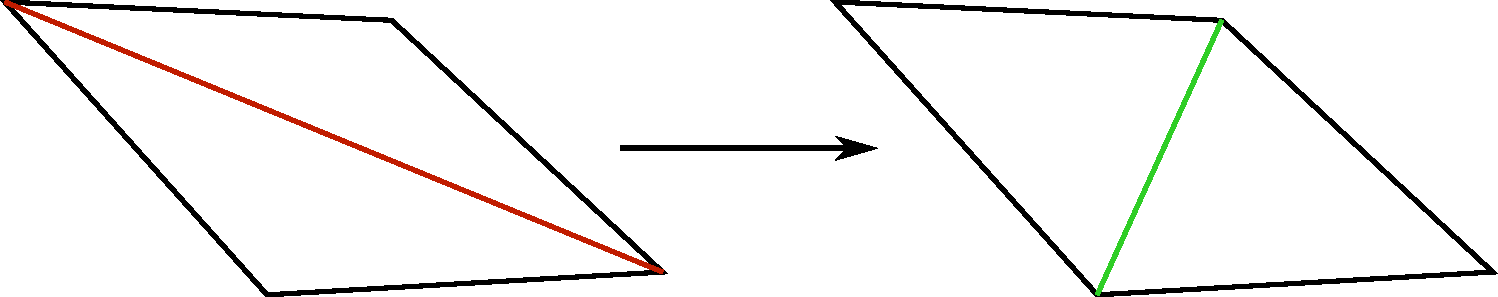
\includegraphics[width=40mm]{image/swap_edge.pdf}};
  \end{tikzpicture}
  }
\end{frame}







% ============================================
% ====== Frame : Validation   ================
% ============================================
\subsection{Validation of the isotropic metric}
\begin{frame}{Validation of the isotropic size map}
  \begin{block}{}
    Polynomial order fixed ($\PolOrder$) $\longrightarrow$ define mesh ($h$-adaptivity)
  \end{block}

  $\Updownarrow$

    \begin{block}{}
    Mesh given ($h$) $\longrightarrow$ define the polynomial order ($p$-adaptivity)
    \end{block}

    \uncover<2->{
      \vspace{-0.4cm}
\setlength{\modelwidth}{6.5cm}
\begin{figure}[!htbp]
  \renewcommand{\modelfile}{image/iso22_mesh}
     \begin{subfigure}[!htbp]{0.5\textwidth}
        \vspace{0.4cm}
        \hspace{-0.5cm}
         \centering
         \begin{tikzpicture}
\pgfmathsetmacro{\xmin} {0.}
\pgfmathsetmacro{\xmax} {9.7}
\pgfmathsetmacro{\zmin} {0.}
\pgfmathsetmacro{\zmax} {2.7}
\pgfmathsetmacro{\zzmax} {3.0}
\pgfmathsetmacro{\xxmax} {10.0}

\begin{axis}[%
width=1.0\modelwidth,
height=0.5\modelwidth,
axis on top, separate axis lines,
xmin=\xmin, xmax=\xxmax, %xlabel={x (km)},
ymin=\zmin, ymax=\zzmax,
yticklabels={},xticklabels={},
y dir=reverse,
point meta min=1.5e3, point meta max=4.6e3,
colorbar/width=2.5mm,
axis x line=top,thick,
axis y line=left,thick,
ylabel style={rotate=-90},
ylabel={$z$},
xlabel={$x$},
ticks = none,
]
\addplot [forget plot] graphics [xmin=\xmin,xmax=\xmax,ymin=\zmin,ymax=\zmax] {{\modelfile}.png};
\end{axis}
\end{tikzpicture}%

         \caption{Marmousi refined mesh at the interfaces (12809 elements).}
         \label{marmousi_mesh_padapt}
     \end{subfigure}
     \hspace{-1cm}
     \renewcommand{\modelfile}{image/iso22_order}
     \renewcommand{\cmapmin}{2}
     \renewcommand{\cmapmax}{4}
     \begin{subfigure}[!htbp]{0.5\textwidth}
        \vspace{-0.3cm}
         \centering
         \begin{tikzpicture}

\pgfmathsetmacro{\xmin} {0.}
\pgfmathsetmacro{\xmax} {9.7}
\pgfmathsetmacro{\zmin} {0.}
\pgfmathsetmacro{\zmax} {2.7}
\pgfmathsetmacro{\zzmax} {3.0}
\pgfmathsetmacro{\xxmax} {10.0}


\begin{axis}[%
width=1.0\modelwidth,
height=0.5\modelwidth,
axis on top, separate axis lines,
xmin=\xmin, xmax=\xxmax, %xlabel={x (km)},
ymin=\zmin, ymax=\zzmax,
yticklabels={},xticklabels={},
y dir=reverse,
colormap/jet, colorbar,
colorbar style={title=\small{order}},
point meta min=\cmapmin, point meta max=\cmapmax,
colorbar/width=2.5mm,
axis x line=top,thick,
axis y line=left,thick,
ylabel style={rotate=-90},
ylabel={$z$},
xlabel={$x$},
ticks = none,
]
\addplot [forget plot] graphics [xmin=\xmin,xmax=\xmax,ymin=\zmin,ymax=\zmax] {{\modelfile}.png};
\end{axis}
\end{tikzpicture}%

         \vspace{-0.9cm}
         \caption{$p$-adaptivity map.}
         \label{marmousi_order_padapt}
     \end{subfigure}

  \begin{tikzpicture}[remember picture,overlay]
    \draw [red,ultra thick,rounded corners, line width=0.1cm] (-6.2,3.45) rectangle (6.3,4.35);
%    \node[xshift=80mm,yshift=-56mm,anchor=north west] at (current page.north west){%
%    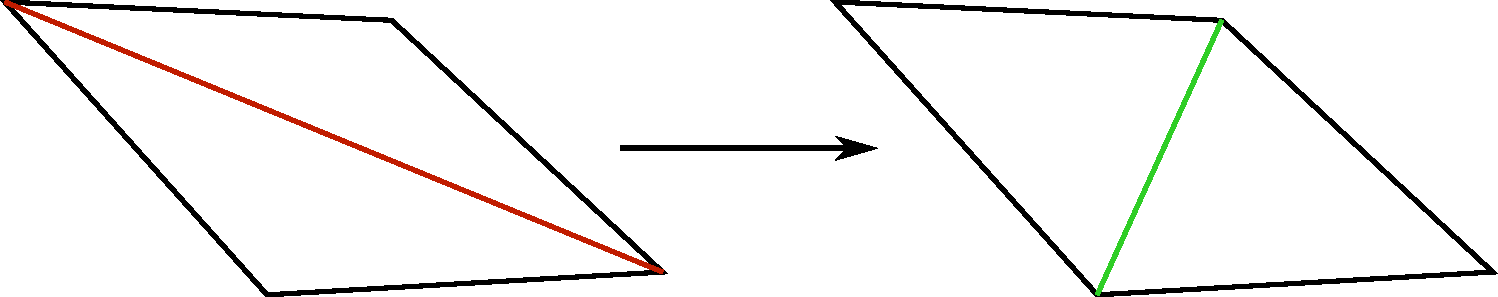
\includegraphics[width=40mm]{image/swap_edge.pdf}};
  \end{tikzpicture}
\end{figure}
     }
     \uncover<3->{
\vspace{-0.5cm}
\begin{table}[!htbp]
  \small
    \centering
    \begin{tabular}{|c|c|c|c|}
    \hline
         $p$-adaptivity    &  P2   & P3   &  P4   \\ \hline
        Number of elements & 1424  & 7981 & 3404   \\ \hline
        Pourcentage        & 11\%  &  63\%&  27\%  \\ \hline
    \end{tabular}
\end{table}
}
\end{frame}


\begin{frame}[noframenumbering]{Validation of the isotropic size map}
  \begin{block}{}
    Polynomial order fixed ($\PolOrder$) $\longrightarrow$ define mesh ($h$-adaptivity)
  \end{block}

  $\Updownarrow$

    \begin{block}{}
    Mesh given ($h$) $\longrightarrow$ define the polynomial order ($p$-adaptivity)
    \end{block}

      \vspace{-0.4cm}
\setlength{\modelwidth}{6.5cm}
\begin{figure}[!htbp]
  \renewcommand{\modelfile}{image/iso22_mesh}
     \begin{subfigure}[!htbp]{0.5\textwidth}
        \vspace{0.4cm}
        \hspace{-0.5cm}
         \centering
         \begin{tikzpicture}
\pgfmathsetmacro{\xmin} {0.}
\pgfmathsetmacro{\xmax} {9.7}
\pgfmathsetmacro{\zmin} {0.}
\pgfmathsetmacro{\zmax} {2.7}
\pgfmathsetmacro{\zzmax} {3.0}
\pgfmathsetmacro{\xxmax} {10.0}

\begin{axis}[%
width=1.0\modelwidth,
height=0.5\modelwidth,
axis on top, separate axis lines,
xmin=\xmin, xmax=\xxmax, %xlabel={x (km)},
ymin=\zmin, ymax=\zzmax,
yticklabels={},xticklabels={},
y dir=reverse,
point meta min=1.5e3, point meta max=4.6e3,
colorbar/width=2.5mm,
axis x line=top,thick,
axis y line=left,thick,
ylabel style={rotate=-90},
ylabel={$z$},
xlabel={$x$},
ticks = none,
]
\addplot [forget plot] graphics [xmin=\xmin,xmax=\xmax,ymin=\zmin,ymax=\zmax] {{\modelfile}.png};
\end{axis}
\end{tikzpicture}%

         \caption{Marmousi refined mesh at the interfaces (12809 elements).}
         \label{marmousi_mesh_padapt}
     \end{subfigure}
     \hspace{-1cm}
     \renewcommand{\modelfile}{image/iso22_order}
     \renewcommand{\cmapmin}{2}
     \renewcommand{\cmapmax}{4}
     \begin{subfigure}[!htbp]{0.5\textwidth}
        \vspace{-0.3cm}
         \centering
         \begin{tikzpicture}

\pgfmathsetmacro{\xmin} {0.}
\pgfmathsetmacro{\xmax} {9.7}
\pgfmathsetmacro{\zmin} {0.}
\pgfmathsetmacro{\zmax} {2.7}
\pgfmathsetmacro{\zzmax} {3.0}
\pgfmathsetmacro{\xxmax} {10.0}


\begin{axis}[%
width=1.0\modelwidth,
height=0.5\modelwidth,
axis on top, separate axis lines,
xmin=\xmin, xmax=\xxmax, %xlabel={x (km)},
ymin=\zmin, ymax=\zzmax,
yticklabels={},xticklabels={},
y dir=reverse,
colormap/jet, colorbar,
colorbar style={title=\small{order}},
point meta min=\cmapmin, point meta max=\cmapmax,
colorbar/width=2.5mm,
axis x line=top,thick,
axis y line=left,thick,
ylabel style={rotate=-90},
ylabel={$z$},
xlabel={$x$},
ticks = none,
]
\addplot [forget plot] graphics [xmin=\xmin,xmax=\xmax,ymin=\zmin,ymax=\zmax] {{\modelfile}.png};
\end{axis}
\end{tikzpicture}%

         \vspace{-0.9cm}
         \caption{$p$-adaptivity map.}
         \label{marmousi_order_padapt}
     \end{subfigure}

  \begin{tikzpicture}[remember picture,overlay]
    \draw [red,ultra thick,rounded corners, line width=0.1cm] (-6.3,3.45) rectangle (6.3,4.35);
%    \node[xshift=80mm,yshift=-56mm,anchor=north west] at (current page.north west){%
%    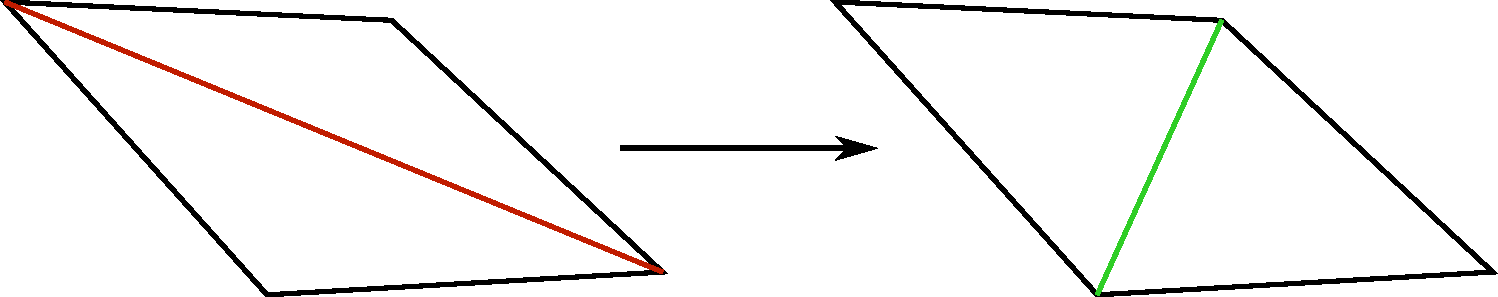
\includegraphics[width=40mm]{image/swap_edge.pdf}};
  \end{tikzpicture}
\end{figure}

\vspace{-0.5cm}
\begin{table}[!htbp]
  \small
    \centering
    \begin{tabular}{|c|c|c|c|c|c|}
    \hline
         & $p$-adaptivity & Full P2 & Full P3 & Full P4 & Full P5 \\ \hline
        L2 relative error & \cellcolor{green!30}0.38\%  & \cellcolor{red!30} 17.40\% & \cellcolor{red!30} 1.44\% & \cellcolor{green!30} 0.30\% &  ref. \\ \hline
        CPU Time (s) & \cellcolor{green!30} 815 & 502 & 1122 & \cellcolor{red!30}2244 & 3455 \\ \hline
    \end{tabular}
\end{table}
\end{frame}



% ============================================
% ====== Frame : Mesh refinement  ============
% ============================================
\subsection{Mesh refinement}
\begin{frame}{Interface refinement}{The metric, a flexible way to define the mesh}
 \small

\begin{overprint}
      \onslide<1>
      \begin{figure}[!htbp]
\centering
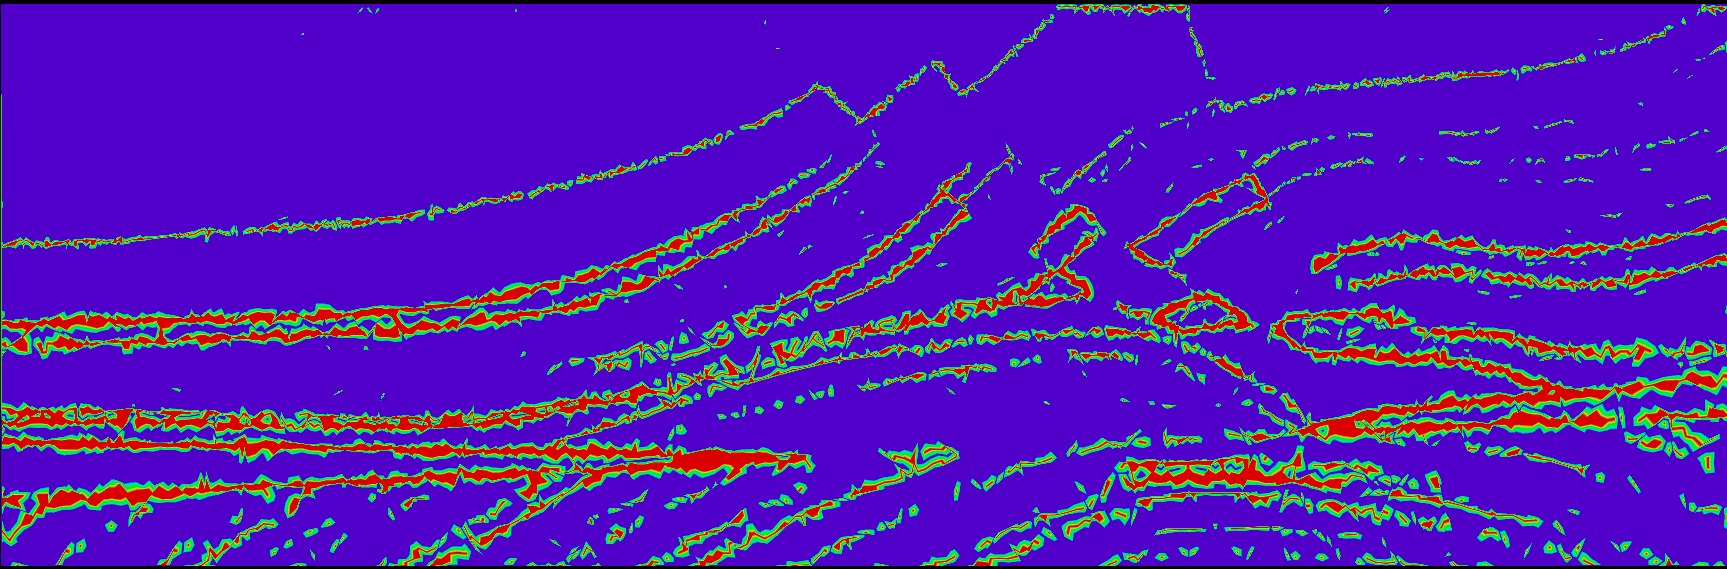
\includegraphics[scale=0.25]{image/grad_e.png}
\caption{Interface detection.}
\label{mesh_marmousi}
\end{figure}
      \onslide<2>
\begin{figure}[!htbp]
\centering
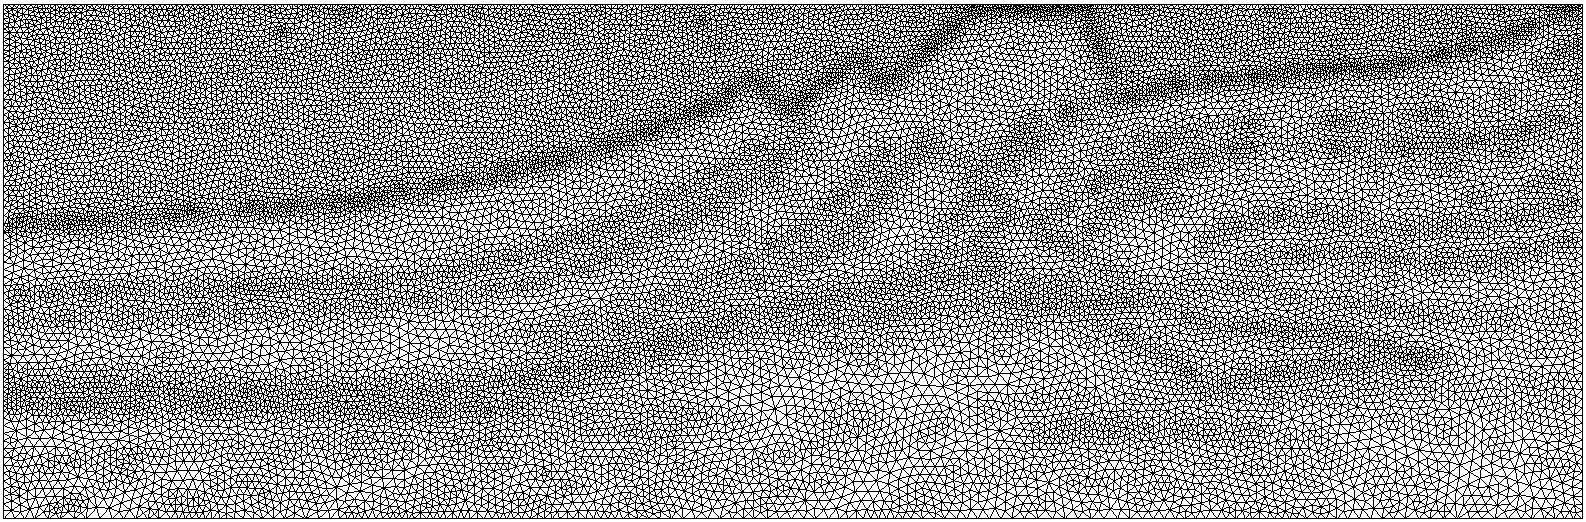
\includegraphics[scale=0.27]{image/marmousi_mesh.png}
\caption{Example of adapted meshes obtained with respect to a size map and taking into account sharp interfaces (42K elements).}
\label{mesh_marmousi}
\end{figure}
    \end{overprint}
\end{frame}




% ============================================
% ====== Frame :  Flowchart into fwi  ========
% ============================================

\subsection{Application to the FWI workflow}
\begin{frame}{Flowchart of remeshing process the FWI course.}

  \begin{figure}[htbp!]
    \vspace{-0.7cm}
  \centering
  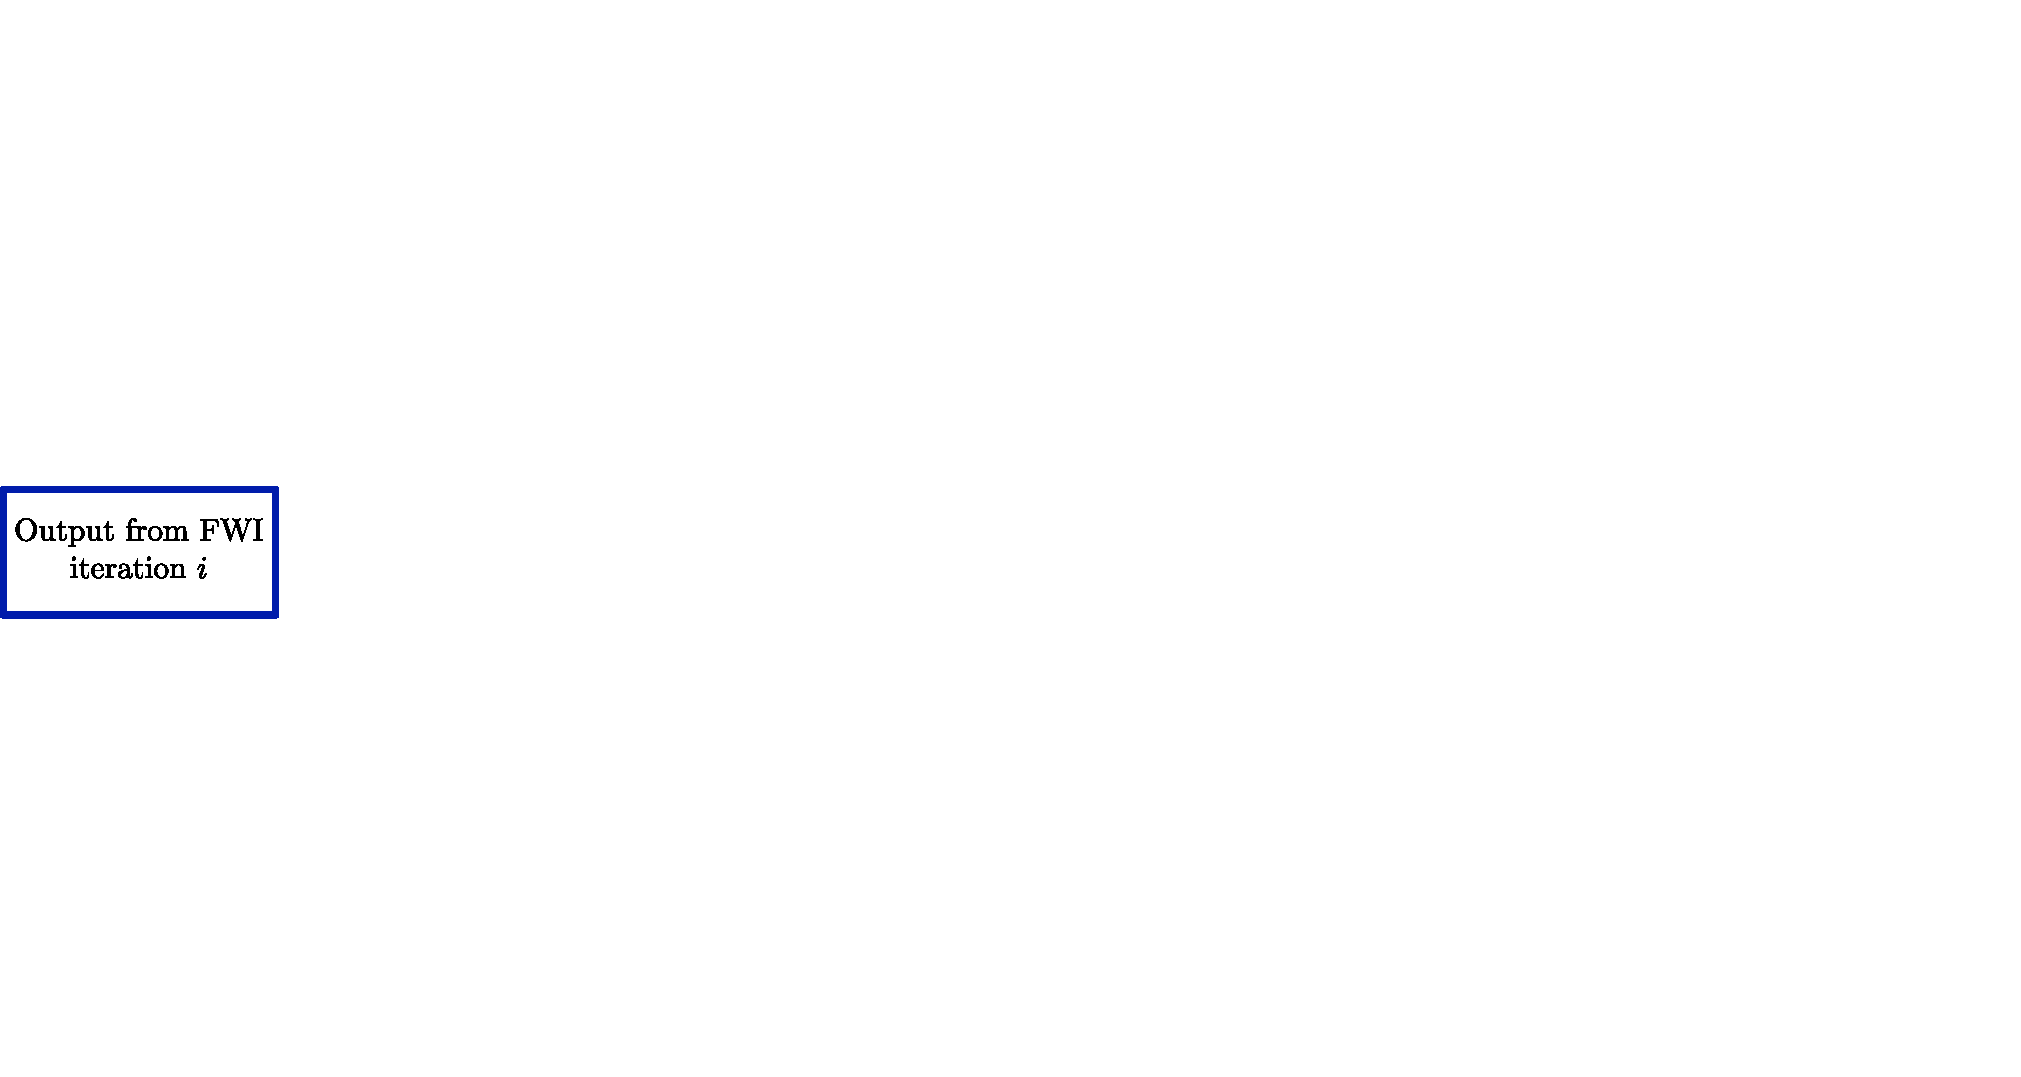
\includegraphics[scale=0.36]{image/remesh_workflow0.pdf}
  \label{flowchart_remesh}
\end{figure}
\end{frame}

\begin{frame}[noframenumbering]{Flowchart of remeshing process the FWI course.}

  \begin{figure}[htbp!]
    \vspace{-0.7cm}
  \centering
  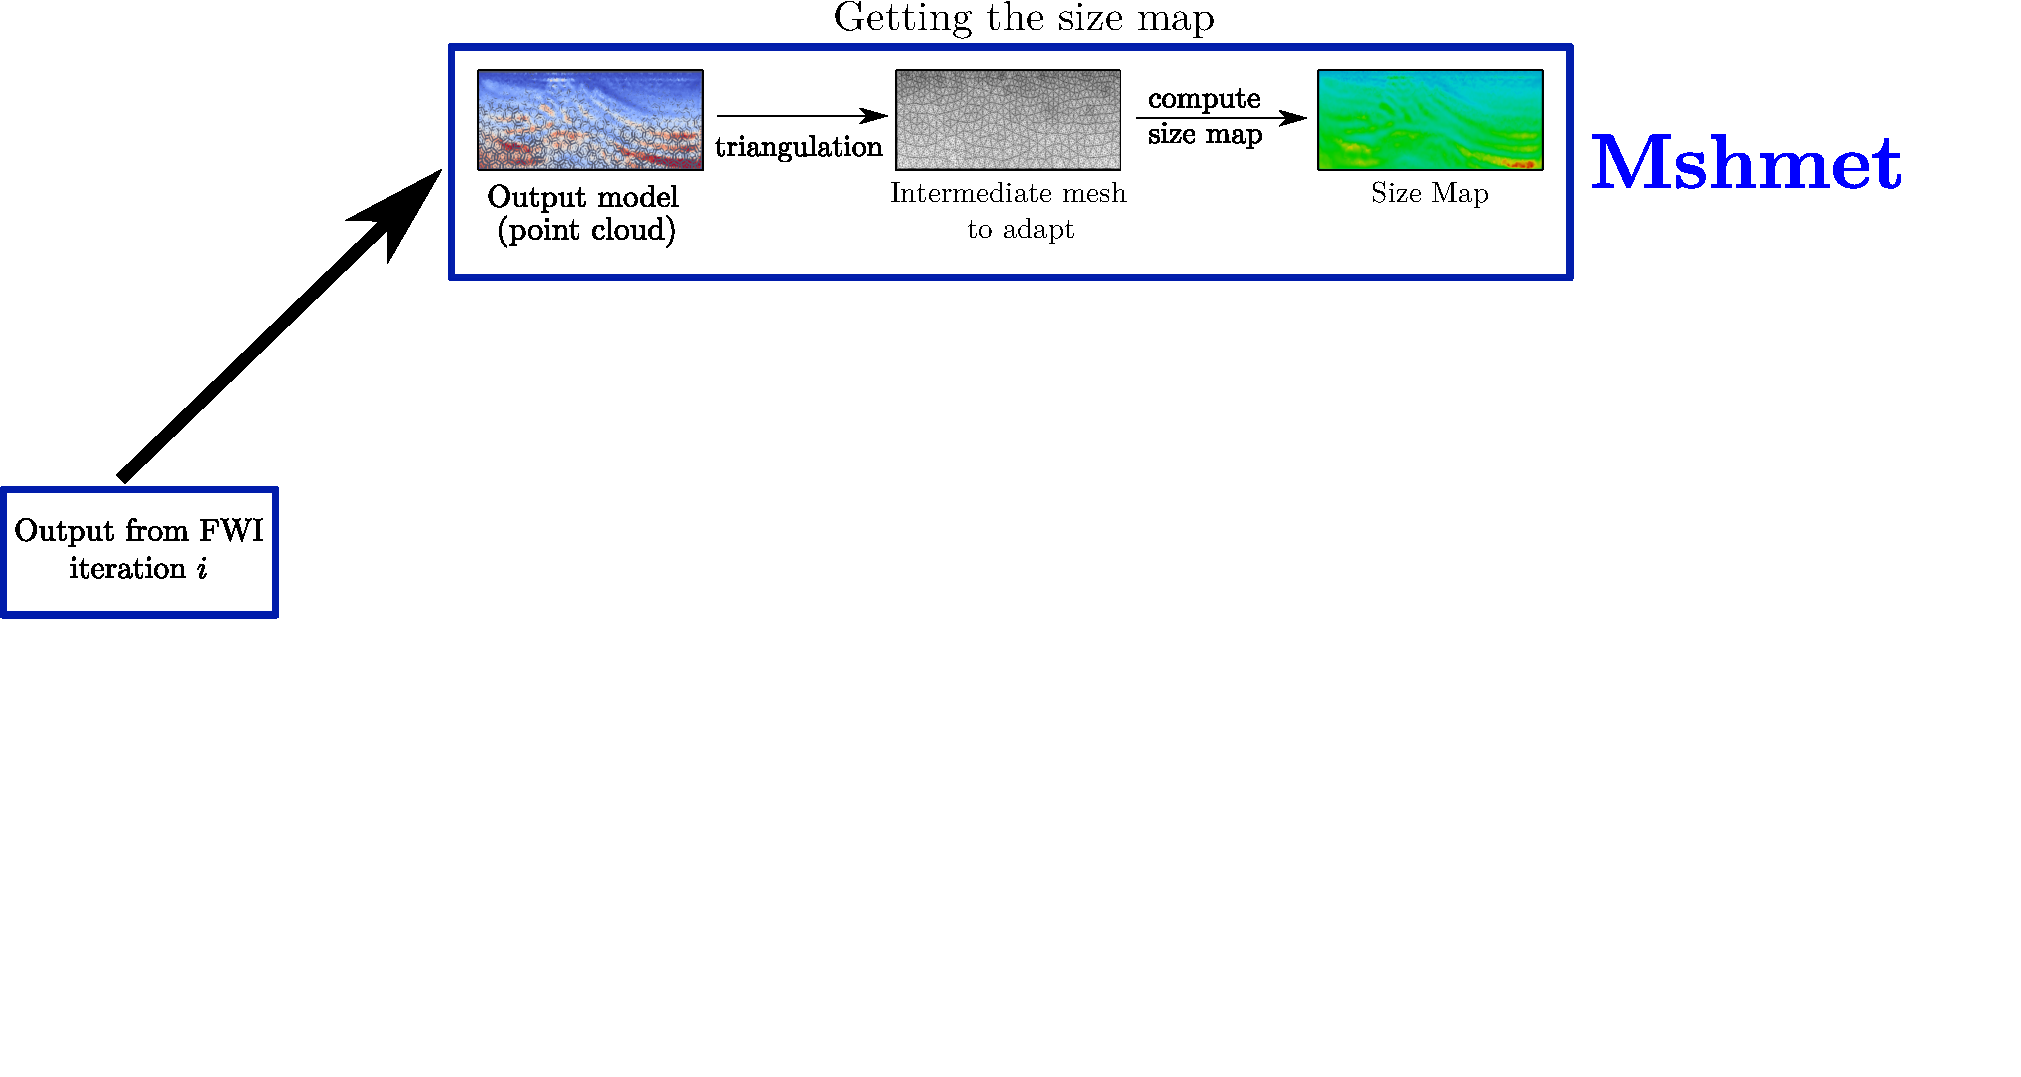
\includegraphics[scale=0.36]{image/remesh_workflow1.pdf}
  \label{flowchart_remesh}
\end{figure}
\end{frame}


\begin{frame}[noframenumbering]{Flowchart of remeshing process the FWI course.}

  \begin{figure}[htbp!]
    \vspace{-0.7cm}
  \centering
  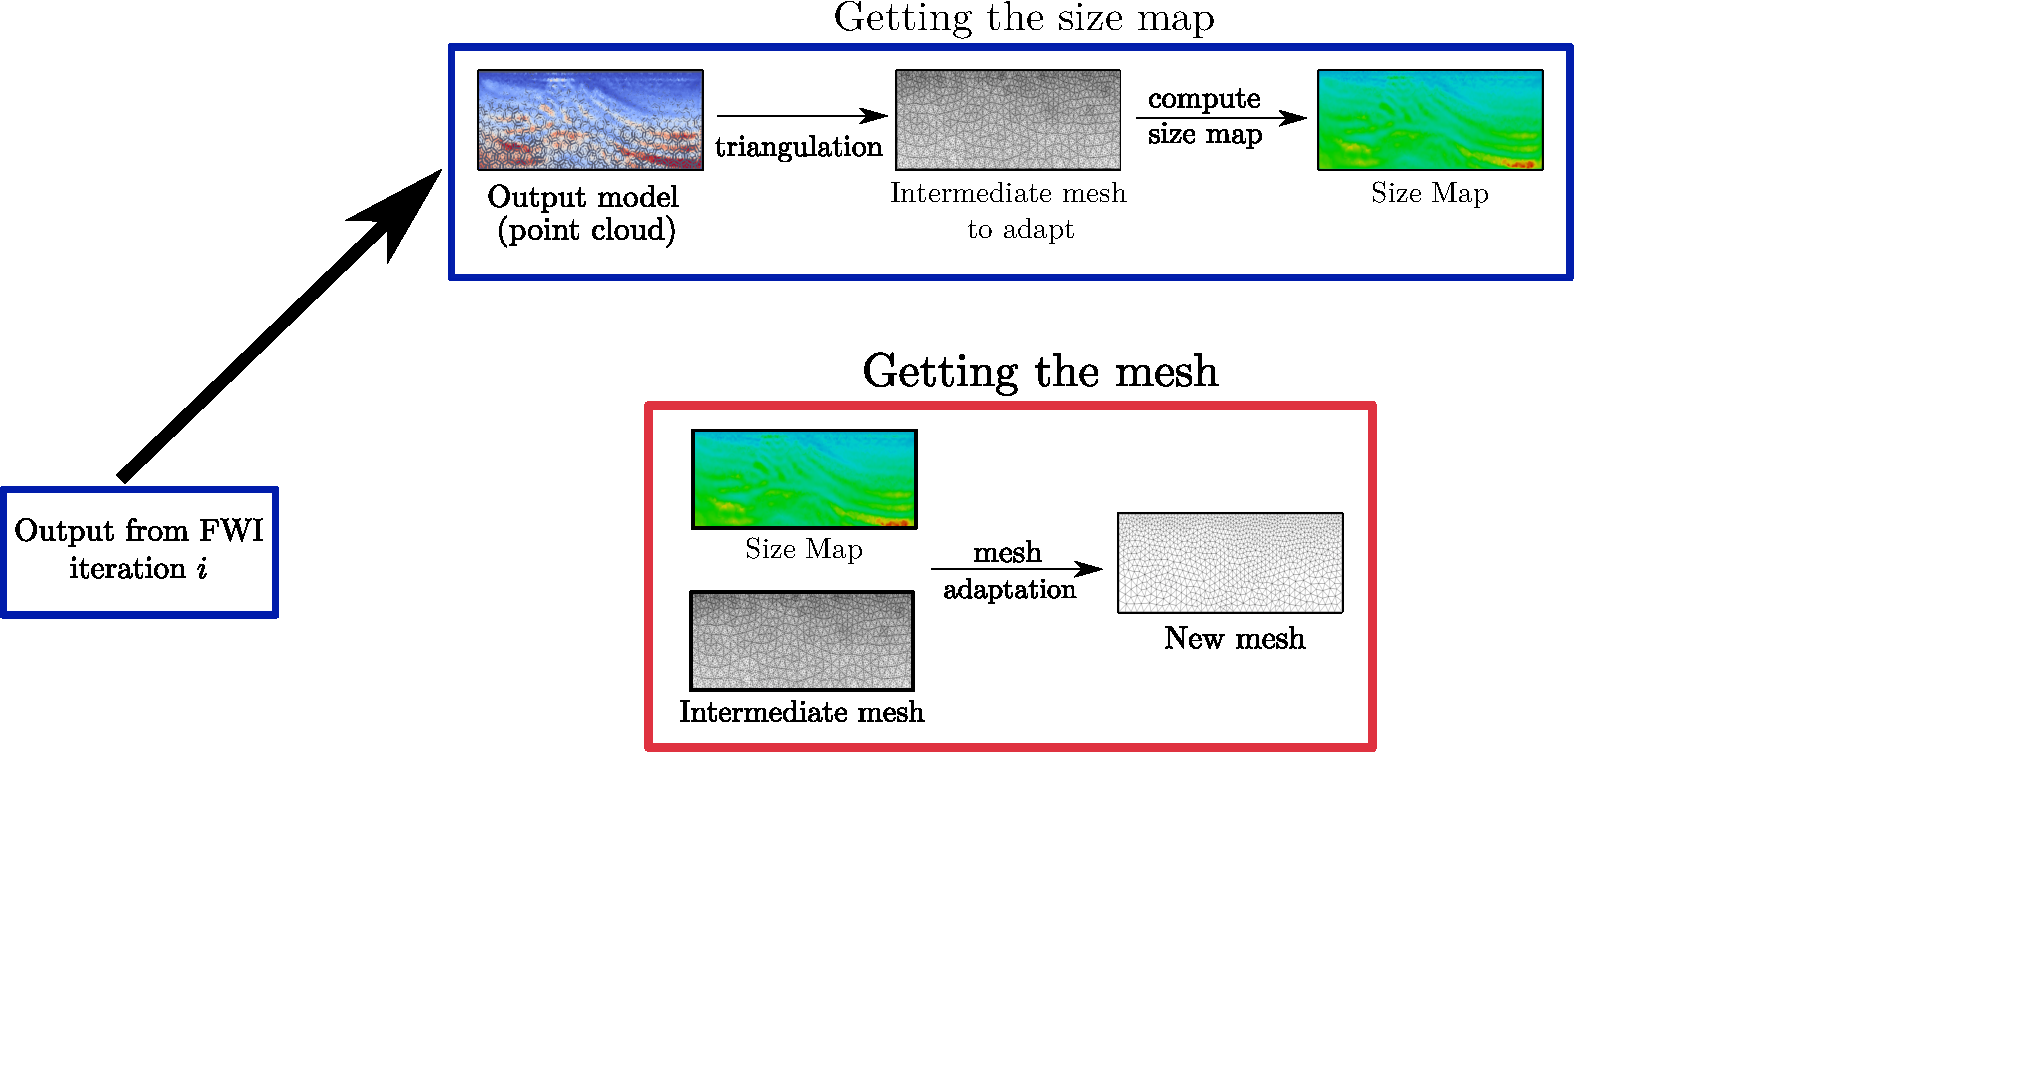
\includegraphics[scale=0.36]{image/remesh_workflow2.pdf}
  \label{flowchart_remesh}
\end{figure}
\end{frame}


\begin{frame}[noframenumbering]{Flowchart of remeshing process the FWI course.}

  \begin{figure}[htbp!]
    \vspace{-0.7cm}
  \centering
  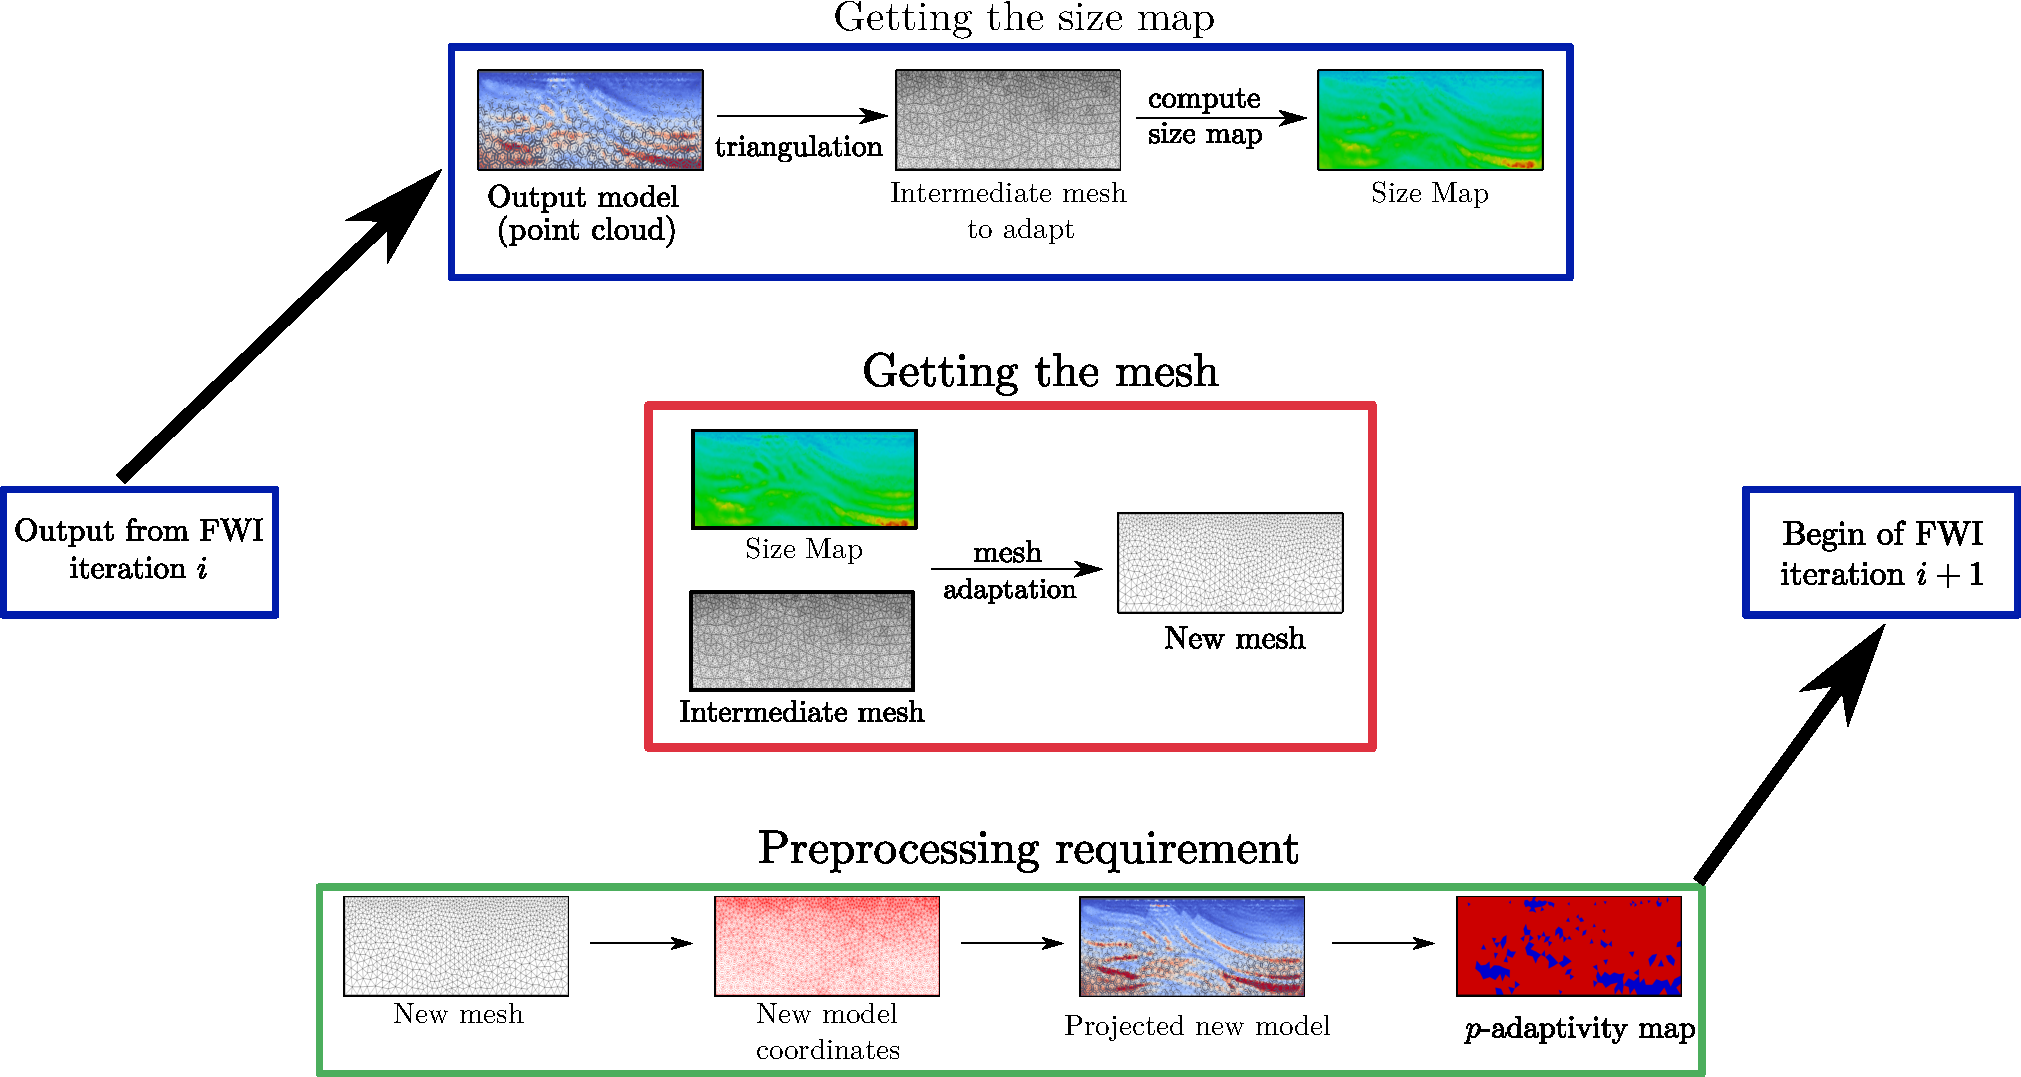
\includegraphics[scale=0.36]{image/remesh_workflow.pdf}
  \label{flowchart_remesh}
\end{figure}
\end{frame}




============================================
====== Frame :  Marmousi constant model ====
============================================

\begin{frame}{Comparaison with Marmousi model}{Constant with constant model per element}
    \vspace{-0.8cm}
  \setlength{\modelwidth}{6.0cm}
  \begin{figure}[!htbp]
    \renewcommand{\modelfile}{image/mesh_adapt/adapt_vp_80}
     \begin{subfigure}[!htbp]{0.5\textwidth}
        \vspace{0.5cm}
        \hspace{-0.5cm}
         \centering
         \begin{tikzpicture}
\pgfmathsetmacro{\xmin} {0.}
\pgfmathsetmacro{\xmax} {9.7}
\pgfmathsetmacro{\zmin} {0.}
\pgfmathsetmacro{\zmax} {2.7}
\pgfmathsetmacro{\zzmax} {3.0}
\pgfmathsetmacro{\xxmax} {10.0}

\begin{axis}[%
width=1.0\modelwidth,
height=0.5\modelwidth,
axis on top, separate axis lines,
xmin=\xmin, xmax=\xxmax, %xlabel={x (km)},
ymin=\zmin, ymax=\zzmax,
yticklabels={},xticklabels={},
y dir=reverse,
point meta min=1.5e3, point meta max=4.6e3,
colorbar/width=2.5mm,
axis x line=top,thick,
axis y line=left,thick,
ylabel style={rotate=-90},
ylabel={$z$},
xlabel={$x$},
ticks = none,
]
\addplot [forget plot] graphics [xmin=\xmin,xmax=\xmax,ymin=\zmin,ymax=\zmax] {{\modelfile}.png};
\end{axis}
\end{tikzpicture}%

         \caption*{Final model \textcolor{\mygreen}{\textbf{with mesh adaptation}}.}
         \label{marmousi_mesh_padapt}
     \end{subfigure}
     \hspace{-1cm}
     \renewcommand{\modelfile}{image/mesh_adapt/classic_vp_80}
     \renewcommand{\cmapmin}{1500}
     \renewcommand{\cmapmax}{5000}
     \begin{subfigure}[!htbp]{0.5\textwidth}
         \centering
         \begin{tikzpicture}
\pgfmathsetmacro{\xmin} {0.}
\pgfmathsetmacro{\xmax} {9.7}
\pgfmathsetmacro{\zmin} {0.}
\pgfmathsetmacro{\zmax} {2.7}
\pgfmathsetmacro{\zzmax} {3.0}
\pgfmathsetmacro{\xxmax} {10.0}


\begin{axis}[%
width=1.0\modelwidth,
height=0.5\modelwidth,
axis on top, separate axis lines,
xmin=\xmin, xmax=\xxmax, %xlabel={x (km)},
ymin=\zmin, ymax=\zzmax,
yticklabels={},xticklabels={},
y dir=reverse,
colormap/paraview, colorbar,
colorbar style={title=\small{$m \cdot s^{-1}$}},
point meta min=\cmapmin, point meta max=\cmapmax,
colorbar/width=2.5mm,
axis x line=top,thick,
axis y line=left,thick,
ylabel style={rotate=-90},
ylabel={$z$},
xlabel={$x$},
ticks = none,
]
\addplot [forget plot] graphics [xmin=\xmin,xmax=\xmax,ymin=\zmin,ymax=\zmax] {{\modelfile}.png};
\end{axis}
\end{tikzpicture}%

         \vspace{-0.6cm}
         \caption*{Final model \textcolor{blue}{\textbf{without mesh adaptation}}.}
     \end{subfigure}
       \end{figure}

  \uncover<2->{
    \scriptsize
\begin{table}[!htbp]
\centering
\begin{tabular}{|l|l|l|l|l|l|}
\hline
& 0-2Hz & 0-5Hz & 0-8Hz & 0-12Hz & 0-15Hz  \\ \hline
\rowcolor{green!30}
Number of elements   & 277    & 779     & 2090    & 4859     & 7065  \\
\rowcolor{green!30}
(with mesh adaptation)      &     &      &     &      &   \\ \hline
\rowcolor{blue!30}
Number of elements      & 7218    & 7218     & 7218    & 7218     & 7218  \\
\rowcolor{blue!30}
(without mesh adaptation)      &     &      &     &      &   \\ \hline
\end{tabular}
\caption{Comparison of the number of elements in the mesh for each frequency band for both strategies.}
\label{nb_elem_mesh_adapt}
\end{table}
}
\end{frame}


\begin{frame}[noframenumbering]{Comparaison with Marmousi model}{Constant with constant model per element}
  \vspace{-0.8cm}
  \setlength{\modelwidth}{6.0cm}
  \begin{figure}[!htbp]
    \renewcommand{\modelfile}{image/mesh_adapt/adapt_vp_80}
     \begin{subfigure}[!htbp]{0.5\textwidth}
        \vspace{0.5cm}
        \hspace{-0.5cm}
         \centering
         \begin{tikzpicture}
\pgfmathsetmacro{\xmin} {0.}
\pgfmathsetmacro{\xmax} {9.7}
\pgfmathsetmacro{\zmin} {0.}
\pgfmathsetmacro{\zmax} {2.7}
\pgfmathsetmacro{\zzmax} {3.0}
\pgfmathsetmacro{\xxmax} {10.0}

\begin{axis}[%
width=1.0\modelwidth,
height=0.5\modelwidth,
axis on top, separate axis lines,
xmin=\xmin, xmax=\xxmax, %xlabel={x (km)},
ymin=\zmin, ymax=\zzmax,
yticklabels={},xticklabels={},
y dir=reverse,
point meta min=1.5e3, point meta max=4.6e3,
colorbar/width=2.5mm,
axis x line=top,thick,
axis y line=left,thick,
ylabel style={rotate=-90},
ylabel={$z$},
xlabel={$x$},
ticks = none,
]
\addplot [forget plot] graphics [xmin=\xmin,xmax=\xmax,ymin=\zmin,ymax=\zmax] {{\modelfile}.png};
\end{axis}
\end{tikzpicture}%

                  \caption*{Final model \textcolor{\mygreen}{\textbf{with mesh adaptation}}.}         \label{marmousi_mesh_padapt}
     \end{subfigure}
     \hspace{-1cm}
     \renewcommand{\modelfile}{image/mesh_adapt/classic_vp_80}
     \renewcommand{\cmapmin}{1500}
     \renewcommand{\cmapmax}{5000}
     \begin{subfigure}[!htbp]{0.5\textwidth}
         \centering
         \begin{tikzpicture}
\pgfmathsetmacro{\xmin} {0.}
\pgfmathsetmacro{\xmax} {9.7}
\pgfmathsetmacro{\zmin} {0.}
\pgfmathsetmacro{\zmax} {2.7}
\pgfmathsetmacro{\zzmax} {3.0}
\pgfmathsetmacro{\xxmax} {10.0}


\begin{axis}[%
width=1.0\modelwidth,
height=0.5\modelwidth,
axis on top, separate axis lines,
xmin=\xmin, xmax=\xxmax, %xlabel={x (km)},
ymin=\zmin, ymax=\zzmax,
yticklabels={},xticklabels={},
y dir=reverse,
colormap/paraview, colorbar,
colorbar style={title=\small{$m \cdot s^{-1}$}},
point meta min=\cmapmin, point meta max=\cmapmax,
colorbar/width=2.5mm,
axis x line=top,thick,
axis y line=left,thick,
ylabel style={rotate=-90},
ylabel={$z$},
xlabel={$x$},
ticks = none,
]
\addplot [forget plot] graphics [xmin=\xmin,xmax=\xmax,ymin=\zmin,ymax=\zmax] {{\modelfile}.png};
\end{axis}
\end{tikzpicture}%

         \vspace{-0.6cm}
         \caption*{Final model \textcolor{blue}{\textbf{without mesh adaptation}}.}
     \end{subfigure}
     \end{figure}

     \scriptsize
\begin{table}[!htbp]
\begin{tabular}{|m{3cm}|l|l|l|l|l|l|}
\hline
& 0-2Hz     & 0-5Hz     & 0-8Hz     & 0-12Hz    & 0-15Hz    & Total \\ \hline
\rowcolor{green!30}
CPU time (h)          & 3         & 11        & 60        & 230       & 408       & 712   \\
\rowcolor{green!30}
(with mesh adaptation)          &          &         &         &        &        &    \\ \hline
\rowcolor{blue!30}
CPU time (h)       & $\sim$432 & $\sim$432 & $\sim$432 & $\sim$432 & $\sim$432 & 2164  \\
\rowcolor{blue!30}
 (without mesh adaptation)       &  &  &  &  &  &   \\ \hline
CPU time ratio \newline (No mesh adapt/mesh adapt)  &  144.0   &    39.3    &   7.2     &    1.9    &   1.1     & \cellcolor{red!30} 3.0   \\ \hline
\end{tabular}
\caption{CPU time comparison between FWI with and without mesh adaptation.}
\label{cpu_tab_1}
\end{table}
\end{frame}



% ============================================
% ====== Frame :  Marmousi WADG model ========
% ============================================

\begin{frame}{Comparaison with Marmousi model}{With WADG parametrization}
  \vspace{-0.8cm}
  \setlength{\modelwidth}{6.0cm}
  \begin{figure}[!htbp]
    \renewcommand{\modelfile}{image/mesh_adapt/wadg_adapt_vp_80}
     \begin{subfigure}[!htbp]{0.5\textwidth}
        \vspace{0.5cm}
        \hspace{-0.5cm}
         \centering
         \begin{tikzpicture}
\pgfmathsetmacro{\xmin} {0.}
\pgfmathsetmacro{\xmax} {9.7}
\pgfmathsetmacro{\zmin} {0.}
\pgfmathsetmacro{\zmax} {2.7}
\pgfmathsetmacro{\zzmax} {3.0}
\pgfmathsetmacro{\xxmax} {10.0}

\begin{axis}[%
width=1.0\modelwidth,
height=0.5\modelwidth,
axis on top, separate axis lines,
xmin=\xmin, xmax=\xxmax, %xlabel={x (km)},
ymin=\zmin, ymax=\zzmax,
yticklabels={},xticklabels={},
y dir=reverse,
point meta min=1.5e3, point meta max=4.6e3,
colorbar/width=2.5mm,
axis x line=top,thick,
axis y line=left,thick,
ylabel style={rotate=-90},
ylabel={$z$},
xlabel={$x$},
ticks = none,
]
\addplot [forget plot] graphics [xmin=\xmin,xmax=\xmax,ymin=\zmin,ymax=\zmax] {{\modelfile}.png};
\end{axis}
\end{tikzpicture}%

         \caption*{Final model \textcolor{\mygreen}{\textbf{with mesh adaptation}}.}
         \label{marmousi_mesh_padapt}
     \end{subfigure}
     \hspace{-1cm}
     \renewcommand{\modelfile}{image/mesh_adapt/wadg_classic_vp_80}
     \renewcommand{\cmapmin}{1500}
     \renewcommand{\cmapmax}{5000}
     \begin{subfigure}[!htbp]{0.5\textwidth}
         \centering
         \begin{tikzpicture}
\pgfmathsetmacro{\xmin} {0.}
\pgfmathsetmacro{\xmax} {9.7}
\pgfmathsetmacro{\zmin} {0.}
\pgfmathsetmacro{\zmax} {2.7}
\pgfmathsetmacro{\zzmax} {3.0}
\pgfmathsetmacro{\xxmax} {10.0}


\begin{axis}[%
width=1.0\modelwidth,
height=0.5\modelwidth,
axis on top, separate axis lines,
xmin=\xmin, xmax=\xxmax, %xlabel={x (km)},
ymin=\zmin, ymax=\zzmax,
yticklabels={},xticklabels={},
y dir=reverse,
colormap/paraview, colorbar,
colorbar style={title=\small{$m \cdot s^{-1}$}},
point meta min=\cmapmin, point meta max=\cmapmax,
colorbar/width=2.5mm,
axis x line=top,thick,
axis y line=left,thick,
ylabel style={rotate=-90},
ylabel={$z$},
xlabel={$x$},
ticks = none,
]
\addplot [forget plot] graphics [xmin=\xmin,xmax=\xmax,ymin=\zmin,ymax=\zmax] {{\modelfile}.png};
\end{axis}
\end{tikzpicture}%

         \vspace{-0.6cm}
                  \caption*{Final model \textcolor{blue}{\textbf{without mesh adaptation}}.}
     \end{subfigure}
  \end{figure}

  \scriptsize
  \begin{table}[!htbp]
\centering
\begin{tabular}{|m{3.5cm}|l|l|l|l|l|}
\hline
& 0-2Hz & 0-5Hz & 0-8Hz & 0-12Hz & 0-15Hz  \\ \hline
\rowcolor{green!30}
Number of elements \newline (with mesh adaptation)      & 277    & 754     & 1958    & 4465     & 6905  \\ \hline
\rowcolor{green!30}
Number of parameters \newline (with mesh adaptation)      & 5263    & 14326     &  37202   & 54340     & 131195  \\ \hline
\rowcolor{blue!30}
Number of elements \newline (without mesh adaptation)      & 7218    & 7218     & 7218    & 7218     & 7218  \\ \hline
\rowcolor{blue!30}
Number of parameters \newline (without mesh adaptation)      & 137142    & 137142     & 137142    & 137142     & 137142  \\ \hline
\end{tabular}
\caption{Number of elements and parameters for each frequency band.}
\label{nb_elem_mesh_adapt_wadg}
\end{table}
\end{frame}


\begin{frame}[noframenumbering]{Comparaison with Marmousi model}{Constant with WADG}
    \vspace{-0.8cm}
  \setlength{\modelwidth}{6.0cm}
  \begin{figure}[!htbp]
    \renewcommand{\modelfile}{image/mesh_adapt/wadg_adapt_vp_80}
     \begin{subfigure}[!htbp]{0.5\textwidth}
        \vspace{0.5cm}
        \hspace{-0.5cm}
         \centering
         \begin{tikzpicture}
\pgfmathsetmacro{\xmin} {0.}
\pgfmathsetmacro{\xmax} {9.7}
\pgfmathsetmacro{\zmin} {0.}
\pgfmathsetmacro{\zmax} {2.7}
\pgfmathsetmacro{\zzmax} {3.0}
\pgfmathsetmacro{\xxmax} {10.0}

\begin{axis}[%
width=1.0\modelwidth,
height=0.5\modelwidth,
axis on top, separate axis lines,
xmin=\xmin, xmax=\xxmax, %xlabel={x (km)},
ymin=\zmin, ymax=\zzmax,
yticklabels={},xticklabels={},
y dir=reverse,
point meta min=1.5e3, point meta max=4.6e3,
colorbar/width=2.5mm,
axis x line=top,thick,
axis y line=left,thick,
ylabel style={rotate=-90},
ylabel={$z$},
xlabel={$x$},
ticks = none,
]
\addplot [forget plot] graphics [xmin=\xmin,xmax=\xmax,ymin=\zmin,ymax=\zmax] {{\modelfile}.png};
\end{axis}
\end{tikzpicture}%

                  \caption*{Final model \textcolor{\mygreen}{\textbf{with mesh adaptation}}.}
         \label{marmousi_mesh_padapt}
     \end{subfigure}
     \hspace{-1cm}
     \renewcommand{\modelfile}{image/mesh_adapt/wadg_classic_vp_80}
     \renewcommand{\cmapmin}{1500}
     \renewcommand{\cmapmax}{5000}
     \begin{subfigure}[!htbp]{0.5\textwidth}
         \centering
         \begin{tikzpicture}
\pgfmathsetmacro{\xmin} {0.}
\pgfmathsetmacro{\xmax} {9.7}
\pgfmathsetmacro{\zmin} {0.}
\pgfmathsetmacro{\zmax} {2.7}
\pgfmathsetmacro{\zzmax} {3.0}
\pgfmathsetmacro{\xxmax} {10.0}


\begin{axis}[%
width=1.0\modelwidth,
height=0.5\modelwidth,
axis on top, separate axis lines,
xmin=\xmin, xmax=\xxmax, %xlabel={x (km)},
ymin=\zmin, ymax=\zzmax,
yticklabels={},xticklabels={},
y dir=reverse,
colormap/paraview, colorbar,
colorbar style={title=\small{$m \cdot s^{-1}$}},
point meta min=\cmapmin, point meta max=\cmapmax,
colorbar/width=2.5mm,
axis x line=top,thick,
axis y line=left,thick,
ylabel style={rotate=-90},
ylabel={$z$},
xlabel={$x$},
ticks = none,
]
\addplot [forget plot] graphics [xmin=\xmin,xmax=\xmax,ymin=\zmin,ymax=\zmax] {{\modelfile}.png};
\end{axis}
\end{tikzpicture}%

         \vspace{-0.6cm}
                  \caption*{Final model \textcolor{blue}{\textbf{without mesh adaptation}}.}
     \end{subfigure}
  \end{figure}

  \scriptsize
\begin{table}[!htbp]
\begin{tabular}{|m{4.0cm}|l|l|l|l|l|l|}
\hline
& 0-2Hz     & 0-5Hz     & 0-8Hz     & 0-12Hz    & 0-15Hz    & Total  \\ \hline
\rowcolor{green!30}
CPU time (h)          & 5         & 22        & 73        & 334       & 541       & 975   \\
\rowcolor{green!30}
(with mesh adaptation)          &          &         &         &        &        &    \\ \hline
\rowcolor{blue!30}
CPU time (h)       & $\sim$730 & $\sim$730 & $\sim$730 & $\sim$730 & $\sim$730 & 3654   \\
\rowcolor{blue!30}
(without mesh adaptation)       &  &  &  &  &  &    \\ \hline
CPU time ratio \newline (without/with mesh adaptation) &  146.0    &    33.2   &   10.0    &    2.2    &   1.3     & \cellcolor{red!30} 3.75   \\ \hline
\end{tabular}
\caption{CPU time comparison between FWI with and without mesh adaptation.}
\label{wadg_cpu_tab}
\end{table}
\end{frame}




% ============================================
% ====== Frame :  Overthrust Mesh Adapt ======
% ============================================




\begin{frame}{Exploit all the DG properties to reconstruct Overthrust 2D model}
 \vspace{-0,8cm}
\setlength{\modelwidth}{6.0cm}
\begin{figure}[!htbp]
  \begin{subfigure}{0.5\textwidth}
    \vspace{0.5cm}
    \hspace{-0.5cm}
\renewcommand{\modelfile}{image/mesh_adapt/overthrust_ini}
\begin{tikzpicture}
  \pgfmathsetmacro{\xmin} {0.}
\pgfmathsetmacro{\xmax} {9.7}
\pgfmathsetmacro{\zmin} {0.}
\pgfmathsetmacro{\zmax} {2.7}
\pgfmathsetmacro{\zzmax} {3.0}
\pgfmathsetmacro{\xxmax} {10.0}

\begin{axis}[%
width=1.0\modelwidth,
height=0.5\modelwidth,
axis on top, separate axis lines,
xmin=\xmin, xmax=\xxmax, %xlabel={x (km)},
ymin=\zmin, ymax=\zzmax,
yticklabels={},xticklabels={},
y dir=reverse,
point meta min=1.5e3, point meta max=5.5e3,
axis x line=top,thick,
axis y line=left,thick,
ylabel style={rotate=-90},
ylabel={$z$},
xlabel={$x$},
ticks = none,
]
\addplot [forget plot] graphics [xmin=\xmin,xmax=\xmax,ymin=\zmin,ymax=\zmax] {{\modelfile}.png};
\end{axis}
\end{tikzpicture}%

\caption*{Blind wavespeed model.}
\label{target_model_2}
\end{subfigure}
\hspace{-1cm}
\begin{subfigure}{0.5\textwidth}
%\vspace{0.2cm}
\renewcommand{\modelfile}{image/mesh_adapt/overthrust}
\renewcommand{\cmapmin}{2500}
\renewcommand{\cmapmax}{5500}
\begin{tikzpicture}
\pgfmathsetmacro{\xmin} {0.}
\pgfmathsetmacro{\xmax} {9.7}
\pgfmathsetmacro{\zmin} {0.}
\pgfmathsetmacro{\zmax} {2.7}
\pgfmathsetmacro{\zzmax} {3.0}
\pgfmathsetmacro{\xxmax} {10.0}


\begin{axis}[%
width=1.0\modelwidth,
height=0.5\modelwidth,
axis on top, separate axis lines,
xmin=\xmin, xmax=\xxmax, %xlabel={x (km)},
ymin=\zmin, ymax=\zzmax,
yticklabels={},xticklabels={},
y dir=reverse,
colormap/paraview, colorbar,
colorbar style={title=\small{$m \cdot s^{-1}$}},
point meta min=\cmapmin, point meta max=\cmapmax,
colorbar/width=2.5mm,
axis x line=top,thick,
axis y line=left,thick,
ylabel style={rotate=-90},
ylabel={$z$},
xlabel={$x$},
ticks = none,
]
\addplot [forget plot] graphics [xmin=\xmin,xmax=\xmax,ymin=\zmin,ymax=\zmax] {{\modelfile}.png};
\end{axis}
\end{tikzpicture}%

\vspace{-0.6cm}
\caption*{Target wavespeed model.}
\label{blind_model_2}
\end{subfigure}
\label{overthrust_ini_and_blind}
\end{figure}

\begin{overprint}
  \onslide<2>
  \scriptsize
  \begin{table}[!htbp]
    \centering
    \begin{tabular}{|l|l|l|l|l|l|}
      \hline
      & 0-2Hz & 0-5Hz & 0-8Hz & 0-12Hz & 0-15Hz                               \\ \hline
      Number of elements $(\nbelem)$   & 391    & 907     &  5144   & 11252     & 1825               \\ \hline
      Number of parameters             & 7429   & 13605   &  36008  & 11252     & 51100              \\ \hline
      Polynomial order $(\PolOrder)$   & 4      & 3       &  2      & 2         & 5                  \\ \hline
      WADG quadrature order $(\QuadOrder)$   & 9      & 7       &  5      & 1         & 11           \\ \hline
      Polynomial basis   & Nodal      & Nodal       &  Nodal      & Nodal         & Bernstein-Bézier \\ \hline
    \end{tabular}
    \label{nb_elem_overthrust}
  \end{table}

  \onslide<3>

  \vspace{-1.0cm}
  \begin{block}{Animation of the reconstruction}
      \begin{center}
      \movie[showcontrols,loop,autostart]
            {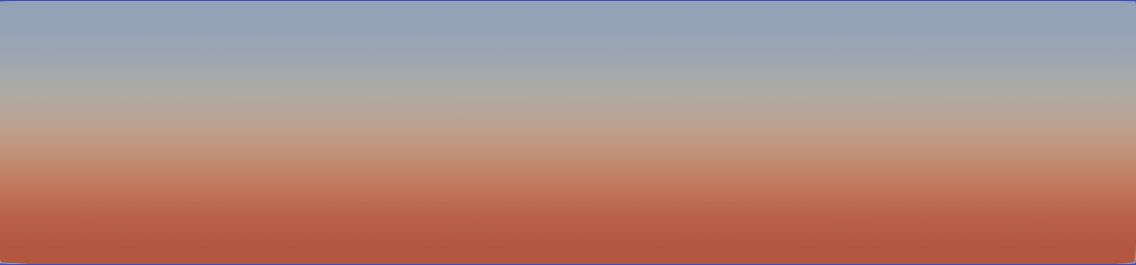
\includegraphics[scale=.3]{animation/overthrust/overthrust_adapt-00.png}}
            {animation/overthrust/out.avi}
      \end{center}
    \end{block}

\end{overprint}

\end{frame}


\begin{frame}{Conclusion}
\end{frame}

\begin{frame}{Perspectives}
  \end{frame}
